\phantomsection
\chapter[Training a Computer to Classify White Blood Cells]{Training a Computer to Classify White Blood Cells\chapsubhead{Phillip Compeau}}
\label{chapter:white_blood_cells}
\renewcommand{\chaptertitle}{Training a Computer to Classify White Blood Cells}
\addcontentsline{cc}{chapter}{Chapter \thechapter} % Adds chapter number to table of contents

%\clearpage \null
%\thispagestyle{empty}
%\AddToShipoutPictureBG*{% Add picture to current page
%  \AtStockLowerLeft{% Add picture to lower-left corner of paper stock
%    \includegraphics[width=\stockwidth]{images/CMYK_ed3/cover/alignment_final}}
%}
%\addtocounter{page}{-1}
%\clearpage

\FloatBarrier

\section{Introduction: How Are Blood Cells Counted?}
\label{sec:introduction}
\phantomsection

Your doctor sometimes counts your blood cells to ensure that they are within healthy ranges as part of a complete blood count. Blood cells consist of \textdef{red blood cells (RBCs)}{red blood cells (RBCs)}{cells in blood that transport oxygen via the hemoglobin protein}, which transport oxygen via the hemoglobin protein, and \textdef{white blood cells (WBCs)}{white blood cells (WBCs)}{cells that help identify and attack foreign cells as part of the immune system}, which help identify and attack foreign cells as part of your immune system.

The classic device used for counting blood cells is the \textdefnogloss{hemocytometer}. In this device, a technician filters a small amount of blood onto a gridded slide and then counts the number of cells of each type in the squares on the grid. As a result, the technician can estimate the number of each type of cell per volume of blood.

\texttt{NEED FIGURE HERE -- TO REPLACE VIDEO}\\

\begin{qbox}[%
Why might the size of the blood sample influence the estimate of blood cell count?
]\end{qbox}

You would not be wrong to think that the hemocytometer seems old-fashioned; it was invented by Louis-Charles Malassez 150 years ago. To reduce the human error inherent in using this device, what if we train a computer to count blood cells for us?

We will focus specifically on WBCs. A low WBC count may indicate a host of diseases that leave the immune system susceptible to attack; a high WBC count may indicate that an infection is present, or that a disease like leukemia has caused overproduction of WBCs.

WBCs divide into families based on their structure and function, and some diseases may cause an abnormally low or high count of a specific WBC classes. We therefore wish not only to identify WBCs in cellular images but also to \textdef{classify}{classification}{the seminal problem of (correctly) categorizing a collection of data} WBCs into their appropriate types.

We will work with a publicly available dataset (hosted at \url{https://github.com/Shenggan/BCCD_Dataset}) containing blood cell images that depict both RBCs and WBCs, as shown in \autoref{fig:three_families}. The cells have been applied with a stain in which a red-orange dye bonds to hemoglobin and a blue dye bonds to DNA and RNA. The red-orange dye will make the RBCs (which do not have DNA or RNA) look red, and the blue dye will make the WBC nuclei look purple.

\autoref{fig:three_families} also illustrates the three main families of WBCs: \textdefnogloss{granulocytes}, \textdefnogloss{lymphocytes}, and \textdefnogloss{monocytes}.  Granulocytes have a \textdef{multilobular nucleus}{multilobular nucleus}{a nucleus consisting of several round ``lobes'' that are linked by thin strands of nuclear material}, which consists of several round ``lobes'' that are linked by thin strands of nuclear material. Monocyte and lymphocyte nuclei only have a single lobe, but the shapes of the nuclei are quite different: lymphocyte nuclei tend to have a more rounded shape (taking up a greater fraction of the cell’s volume), whereas monocyte nuclei have a more irregular shape.\\

\begin{figure}[h]
\centering
\tabcolsep = 1em
\mySfFamily
\begin{tabular}{c c c}
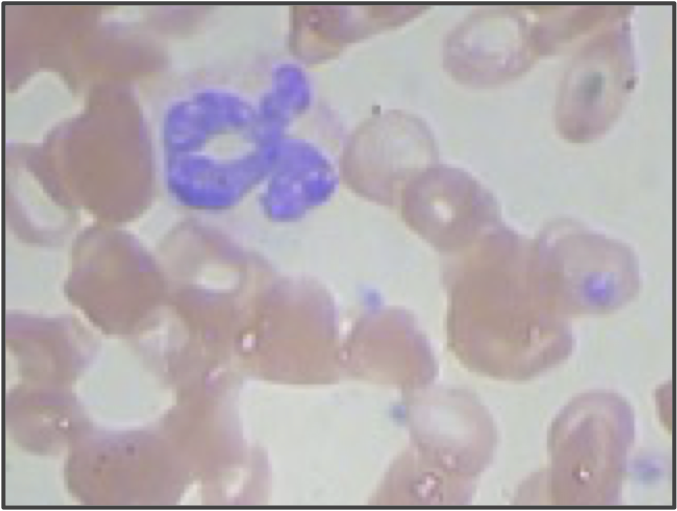
\includegraphics[width = 0.25\textwidth]{../images/neutrophil.png} & 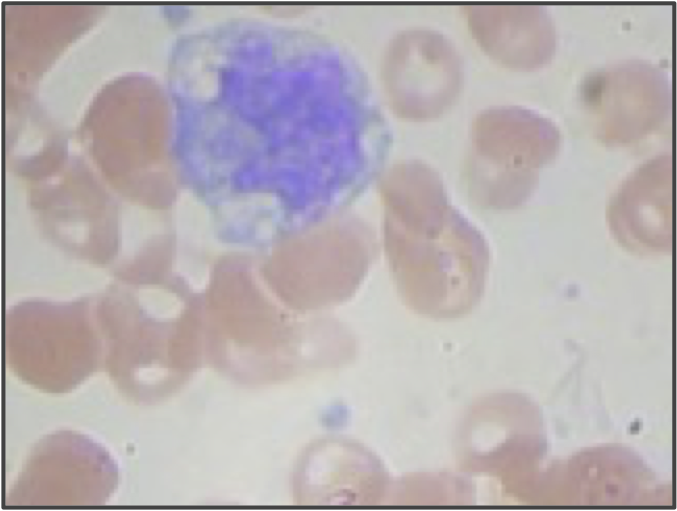
\includegraphics[width = 0.25\textwidth]{../images/monocyte.png} & 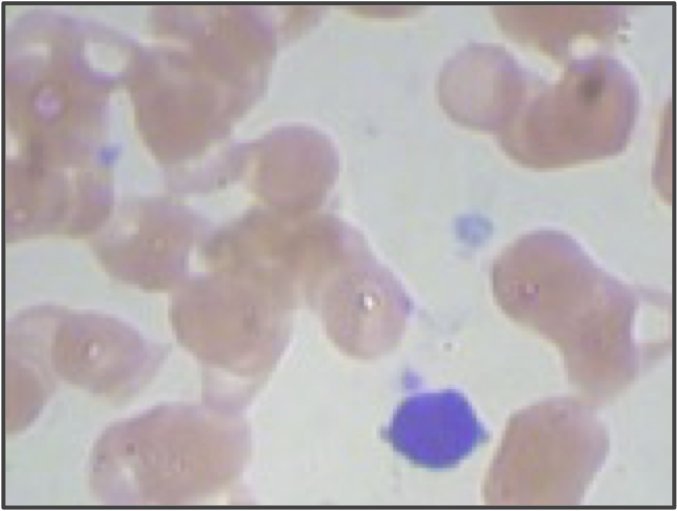
\includegraphics[width = 0.25\textwidth]{../images/lymphocyte.png}
\end{tabular}
\caption{Three images from the blood cell image dataset showing three types of WBCs. In our dataset, these cells correspond to image IDs 3, 15, and 20. (Left) A specific subtype of granulocyte called a neutrophil, illustrating the multilobular structure of this WBC family. (Center) A monocyte with a single, irregularly-shaped nucleus. (Right) A lymphocyte with a small, round nucleus.}
\label{fig:three_families}
\end{figure}

In this module, our goal is twofold. First, can we excise, or \textdef{segment}{segmentation}{the process of partitioning an image in order to excise objects of interest}, WBCs from these cellular images? Second, can we train a computer to classify WBCs by family? To perform these tasks, we will enlist CellOrganizer (\url{http://www.cellorganizer.org}), a powerful software resource that can perform a wide variety of automated analyses on cellular images.

When you look at the cells in the figure above, you may think that our two tasks will be easy. Identifying WBCs only requires identifying the large purplish regions, and classifying them is just a matter of categorizing them according to the differences in shape that we described above. Yet even after decades of research into computer vision, researchers struggle to attain the precision of the human eye.

\FloatBarrier
\phantomsection

\section{Segmenting White Blood Cell Images}
\label{sec:segmenting_white_blood_cell_images}
\phantomsection
\subsection{Image segmentation requires a tailored approach}

We begin our work by discussing how to segment WBCs from an image of blood cells like the ones in \autoref{fig:three_families}. Researchers have developed many algorithms for cellular image segmentation, but no single approach can be used in all contexts. We therefore will identify the key attributes that make this dataset special and then use these features to develop our own segmentation algorithm.

We ask what makes the WBC nucleus so easy for a human to spot in the images in \autoref{fig:three_families}. You may be screaming, ``The nucleus is dark blue! How hard could it be?'' But to train a computer to segment images by color, we should first understand how the computer represents color in images.

\FloatBarrier
\phantomsection
\subsection{The RGB color model}

In the \textdef{RGB color model}{RGB color model}{a model in which every rectangular pixel on a computer screen receives a solid color formed as a mixture of red, green, and blue}, every rectangular pixel on a computer screen receives a solid color formed as a mixture of the three primary colors of light: red, green, and blue (hence the acronym ``RGB''). The amount of each color in a pixel is expressed as an integer between 0 and 255, inclusively, where larger integers correspond to larger amounts of the color.

A few colors are shown in \autoref{fig:RGB_color_chart} along with their RGB equivalents; for example, magenta corresponds to equal parts red and blue. Note that a color like (128, 0, 0) contains only red but appears duskier than (256, 0, 0) because the red has not been “turned on” fully.

\begin{figure}[h]
\centering
\mySfFamily
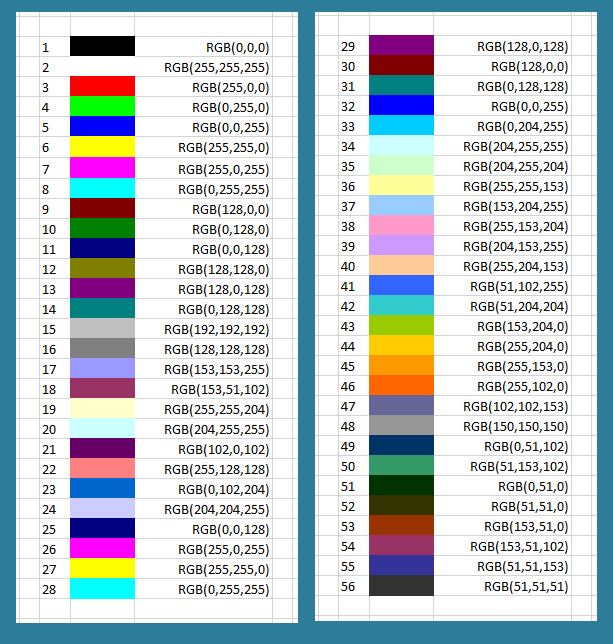
\includegraphics[width = 0.6\textwidth]{../images/RGB_color_chart.png}
\caption{A collection of colors along with their RGB codes. This table corresponds to mixing colors of light instead of pigment, which causes some non-intuitive effects; for example, yellow is formed by mixing equal parts red and green. The last six colors appear muted because they only receive half of a given color value compared to a color that receives 256 units. If all three colors are mixed in equal proportions, then we obtain a color on the gray scale between white (maximum amount of all three colors) and black (no color). Source: https://excelatfinance.com/xlf/xlf-colors-1.php; Excel at Finance.}
\label{fig:RGB_color_chart}
\end{figure}

The RGB model gives us an idea for finding a WBC nucleus. If we scan through the pixels in a blood cell image, we can “turn off” any pixels whose RGB color values are not sufficiently blue.\\

\begin{qbox}[%
You can find a color picker in \texttt{Utilities > Digital Color Meter} (Mac OS X) or by using ShareX for Windows. Open your color picker, and hover the picker over different parts of the the granulocyte image above. What are the typical RGB values for the WBC nucleus, and how do these RGB values differ from both the RBCs and the background of the image?
]\end{qbox}

\FloatBarrier
\phantomsection
\subsection{Binarizing an image based on a color threshold}

Using a color picker, we find (unsurprisingly) that the blue values for pixels inside a stained WBC nucleus are higher than those of the surrounding RBCs. We will therefore \textdefnogloss{binarize} our image by coloring a pixel white (RGB: (256, 256, 256)) if its blue value is above some threshold, and turning a pixel black (RGB: (0, 0, 0)) if its blue value is beneath some threshold.

The binarized version of the cellular image from \autoref{fig:three_families} (left) for the threshold value of 153 is shown in \autoref{fig:neutrophil_binarized_blue}. Unfortunately, we cannot clearly see the WBC nucleus in this binarized image because although the nucleus has high blue values, so does the image's background, since light colors are formed by mixing high percentages of red, green, and blue.

\begin{figure}[h]
\centering
\mySfFamily
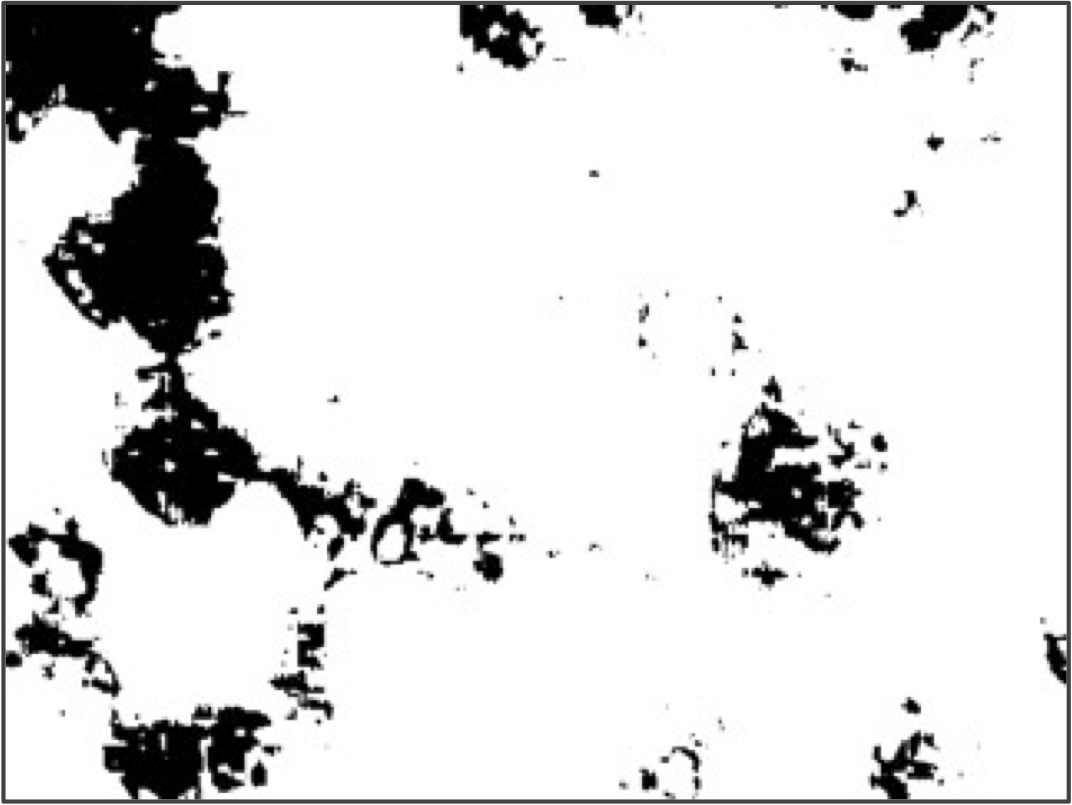
\includegraphics[width = 0.25\textwidth]{../images/neutrophil_binarized_blue.png}
\caption{A binarized version of the granulocyte from \autoref{fig:three_families} (left) (having image ID 3 in our dataset). A pixel is colored white if it has a blue value of 153 or greater, and the pixel is colored black otherwise. The region with the nucleus is not clearly visible because much of the background of the image, which is very light, also has a high blue value.}
\label{fig:neutrophil_binarized_blue}
\end{figure}

\begin{qbox}[%
How might we modify our segmentation approach to perform a binarization that identifies the WBC nucleus more effectively?
]\end{qbox}

We were unable to distinguish between the image background and the WBC nucleus using blue color values, but a color picker verifies that WBC nuclear pixels have a green content that is much lower than the background and a red content that is lower than every other part of the image. \autoref{fig:neutrophil_binarized_other_colors} shows two binarizations of the original image using a green threshold of 153 and a red threshold of 166.

\begin{figure}[h]
\centering
 \tabcolsep = 1em
\mySfFamily
\begin{tabular}{c c}
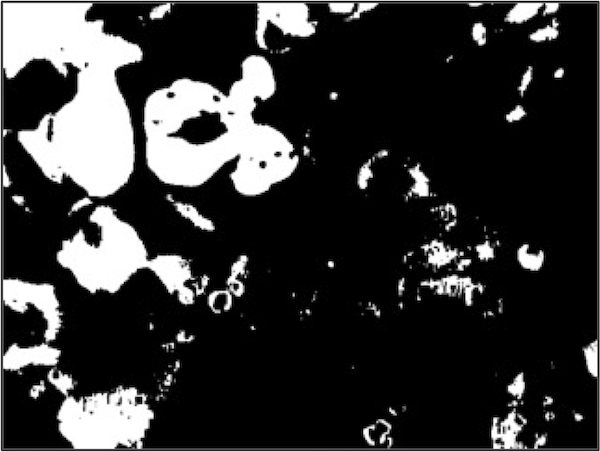
\includegraphics[width = 0.25\textwidth]{../images/neutrophil_binarized_green.png} & 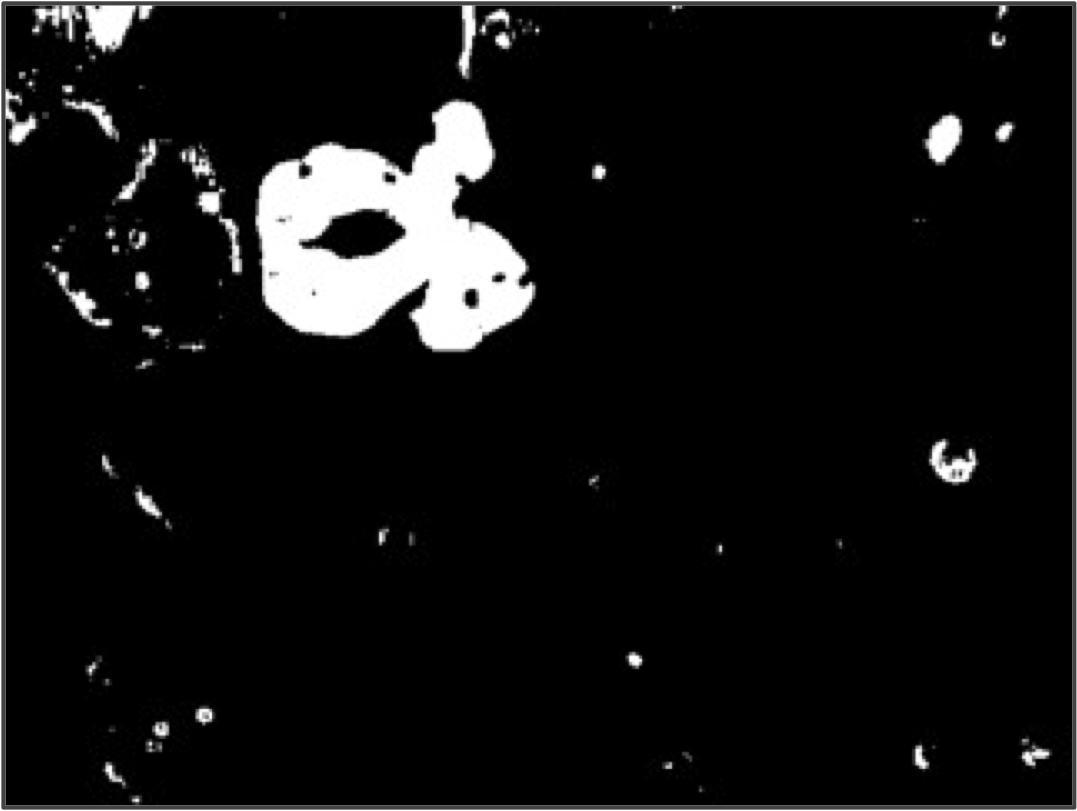
\includegraphics[width = 0.25\textwidth]{../images/neutrophil_binarized_red.png}
\end{tabular}
\caption{Two more binarized versions of the neutrophil image from \autoref{fig:three_families} (left), based on the green and red channels. For both of these colors, the WBC nucleus tends to have lower values than other parts of the original image. (Left) A binarization in which a pixel is turned white if it has a green value less than or equal to 153. (Right) A binarization in which a pixel is turned white if it has a red value less than or equal to 166.}
\label{fig:neutrophil_binarized_other_colors}
\end{figure}

It would seem that we should work with the binarized image based on the red threshold, which contains the clearest image of the nucleus among the three binarized images. However, note that each threshold was successful in eliminating some of the non-nuclear parts of the image. For example, consider the white blob in the top left of the binarized image based on the red threshold in \autoref{fig:neutrophil_binarized_other_colors} (right).

This insight gives us an idea: if each of the three images is successful at excluding some part of the image, then let us produce a fourth image such that a pixel is white if it is white in all three binarized images.\tutorial[https://biologicalmodeling.org/white_blood_cells/tutorial_nuclear_segmentation]

\FloatBarrier
\phantomsection
\subsection{Successful segmentation is subject to parameters}

If we segment all of the images in the dataset via the process described above, then we typically obtain a nice result, as indicated in \autoref{fig:segmentation} for the sample monocyte and lymphocyte images presented in the [introduction](home). Even though these images have been binarized, the large irregular shape of the monocyte nucleus and the small round shape of the lymphocyte nucleus are still visible.

\begin{figure}[h]
\centering
\tabcolsep = 1em
\mySfFamily
\begin{tabular}{c c}
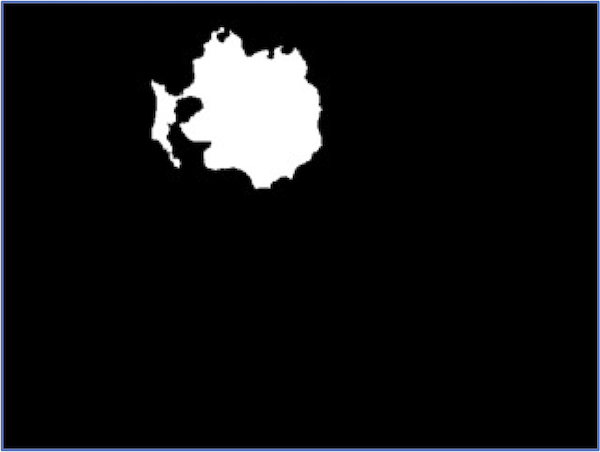
\includegraphics[width = 0.25\textwidth]{../images/monocyte_binarized.png} & 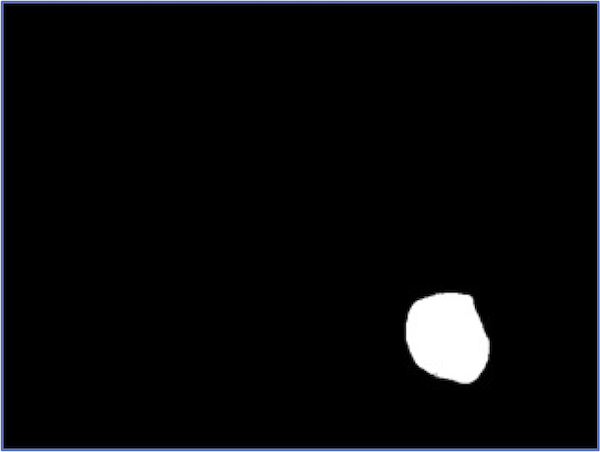
\includegraphics[width = 0.25\textwidth]{../images/lymphocyte_binarized.png}
\end{tabular}
\caption{Image segmentation of the monocyte (left) and lymphocyte (right) corresponding to IDs 15 and 20 in the provided dataset.}
\label{fig:segmentation}
\end{figure}

This is not to say that our segmentation pipeline is perfect. \autoref{fig:segmentation_imperfect} illustrates that for a few images in our dataset, we may not correctly segment the entire nucleus.

\begin{figure}[h]
\centering
\tabcolsep = 1em
\mySfFamily
\begin{tabular}{c c}
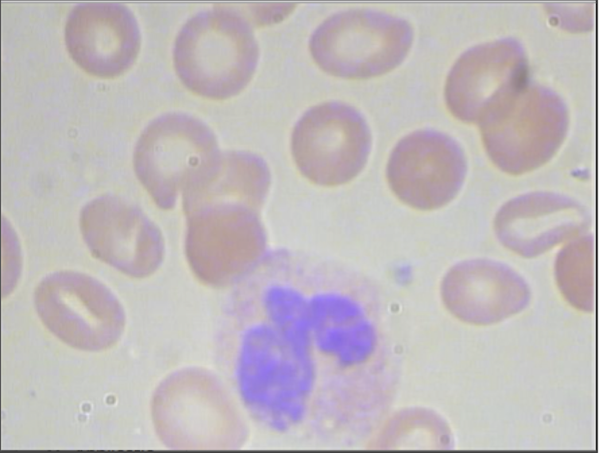
\includegraphics[width = 0.25\textwidth]{../images/WBC_167.png} & 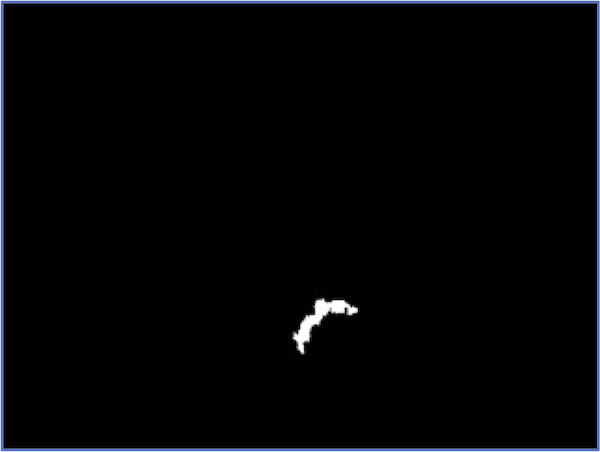
\includegraphics[width = 0.25\textwidth]{../images/WBC_167_segmentation.png}
\end{tabular}
\caption{(Left) An image of a WBC (ID: 167). (Right) The binarization of this image, showing that the nucleus is not correctly identified during segmentation using the parameters described in this section.}
\label{fig:segmentation_imperfect}
\end{figure}

We can continue to tweak threshold parameters, but our relatively simple algorithm has successfully segmented most of the WBC nuclei from our dataset. We are ready to move on to classifying WBC nuclei into families according to their shape.

\FloatBarrier
\phantomsection
\section{An Overview of Classification and k-Nearest Neighbors}
\label{sec:knn}


\phantomsection
\subsection{The classification problem}

Labeling images of WBCs according to their family is a specific instance of an ubiqitous problem in data science, in which we wish to classify each object in a given dataset into one of \textvar{k} classes.

In our ongoing example, the data are images of WBCs, and the classes are the three main families of WBCs (granulocytes, lymphocytes, and monocytes). To take a different example, our data could be tumor genomes sequenced from cancer patients, which we want to classify based on which therapeutic should be prescribed for the patient. Or the data may be the past sales behavior of shoppers, who we want to classify into two classes based on a prediction of whether they will buy a new product.

\FloatBarrier
\phantomsection
\subsection{The iris flower dataset}

A classical dataset commonly used for motivating classification is the \textdef{iris flower dataset}{iris flower dataset}{a dataset commonly used for motivating classification, which was compiled by Edgar Anderson, and which Ronald Fisher used in a seminal paper on classification in 1936}, which was compiled by Edgar Anderson, and which Ronald Fisher used in a seminal paper on classification in 1936. Anderson took measurements from 150 iris flowers, equally divided among three species (\autoref{fig:iris_flowers}).\\

\begin{figure}[h]
\centering
\tabcolsep = 1em
\mySfFamily
\begin{tabular}{c c c}
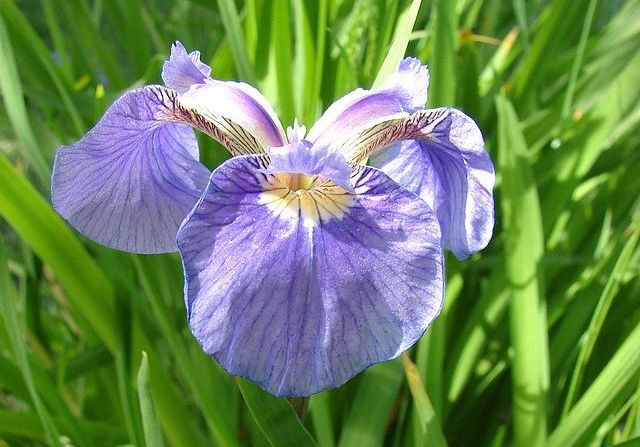
\includegraphics[width = 0.25\textwidth]{../images/Iris_setosa_2.jpg} & 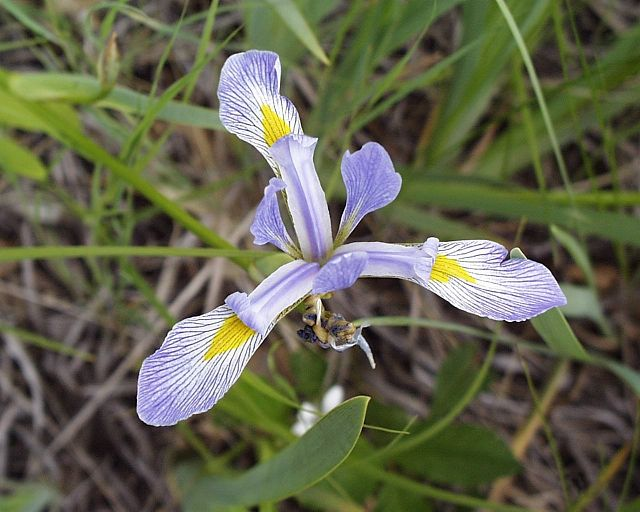
\includegraphics[width = 0.25\textwidth]{../images/Iris_versicolor.jpg} & 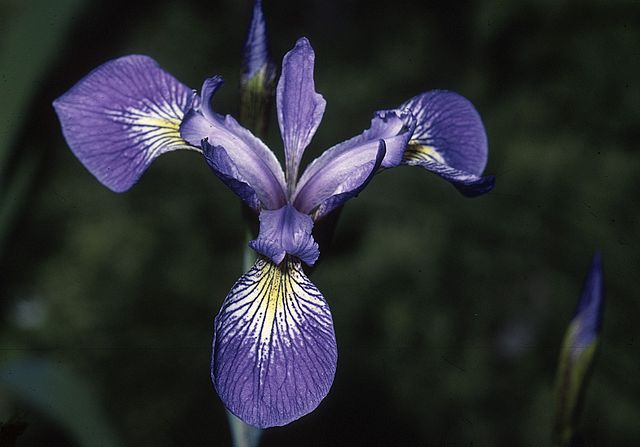
\includegraphics[width = 0.25\textwidth]{../images/Iris_virginica.jpg}
\end{tabular}
\caption{Representative images of the three species of iris included in Anderson's iris flower dataset. (Left) \textit{Iris setosa}. (Center)  \textit{Iris versicolor}. (Right) \textit{Iris virginica}.}
\label{fig:iris_flowers}
\end{figure}

Anderson measured four attributes, or \textdef{features}{feature}{a measurable characteristic of a data point; multiple features are grouped together to form a feature vector in which the \textvar{i}-th element is the data point's value for the \textvar{i}-th feature}, of each of the flowers in his dataset: both the width and height of the flower's petal, and both the width and height of the flower's sepal (a green offshoot beneath the petals). The features and species labels for twelve of the flowers in the iris flower dataset are shown in \autoref{fig:iris_feature_table}. Fisher considered whether it was possible to classify each flower according to its species using only the features Anderson had measured.\\

\begin{figure}[h]
\centering
\tabcolsep = 1 em
\mySfFamily
\begin{tabular}{c c c c c}
\textbf{Sepal length} & \textbf{Sepal width} & \textbf{Petal length} & \textbf{Petal width} & \textbf{Species} \\
5.1 & 3.5 & 1.4 & 0.2 & \textit{I. setosa} \\
4.9 & 3.0 & 1.4 & 0.2 & \textit{I. setosa} \\
4.7 & 3.2 & 1.3 & 0.2 & \textit{I. setosa} \\
4.6 & 3.1 & 1.5 & 0.2 & \textit{I. setosa} \\
7.0 & 3.2 & 4.7 & 1.4 & \textit{I. versicolor} \\
6.4 & 3.2 & 4.5 & 1.5 & \textit{I. versicolor} \\
6.9 & 3.1 & 4.9 & 1.5 & \textit{I. versicolor} \\
5.5 & 2.3 & 4.0 & 1.3 & \textit{I. versicolor} \\
6.3 & 3.3 & 6.0 & 2.5 & \textit{I. virginica} \\
5.8 & 2.7 & 5.1 & 1.9 & \textit{I. virginica} \\
7.1 & 3.0 & 5.9 & 2.1 & \textit{I. virginica} \\
6.3 & 2.9 & 5.6 & 1.8 & \textit{I. virginica} \\
\end{tabular}
\caption{A table containing values of the four features for twelve members of the iris flower dataset, along with each flower's species. Distances are in centimeters. The complete dataset was accessed from the University of California, Irvine Machine Learning Repository.}
\label{fig:iris_feature_table}
\end{figure}

\begin{qbox}[%
What characteristics do flowers from each species tend to share in terms of the four features in \autoref{fig:iris_feature_table}?
]\end{qbox}

\FloatBarrier
\phantomsection
\subsection{From flowers to vectors}

If we were to use only two features in the Iris flower dataset, then a flower's feature values \textvar{x} and \textvar{y} could be represented as a point in two-dimensional space $(x, y)$. \autoref{fig:iris_petal_data} shows such a plot for the features of petal length (x-axis) and petal width (y-axis).

\begin{figure}[h]
\centering
\mySfFamily
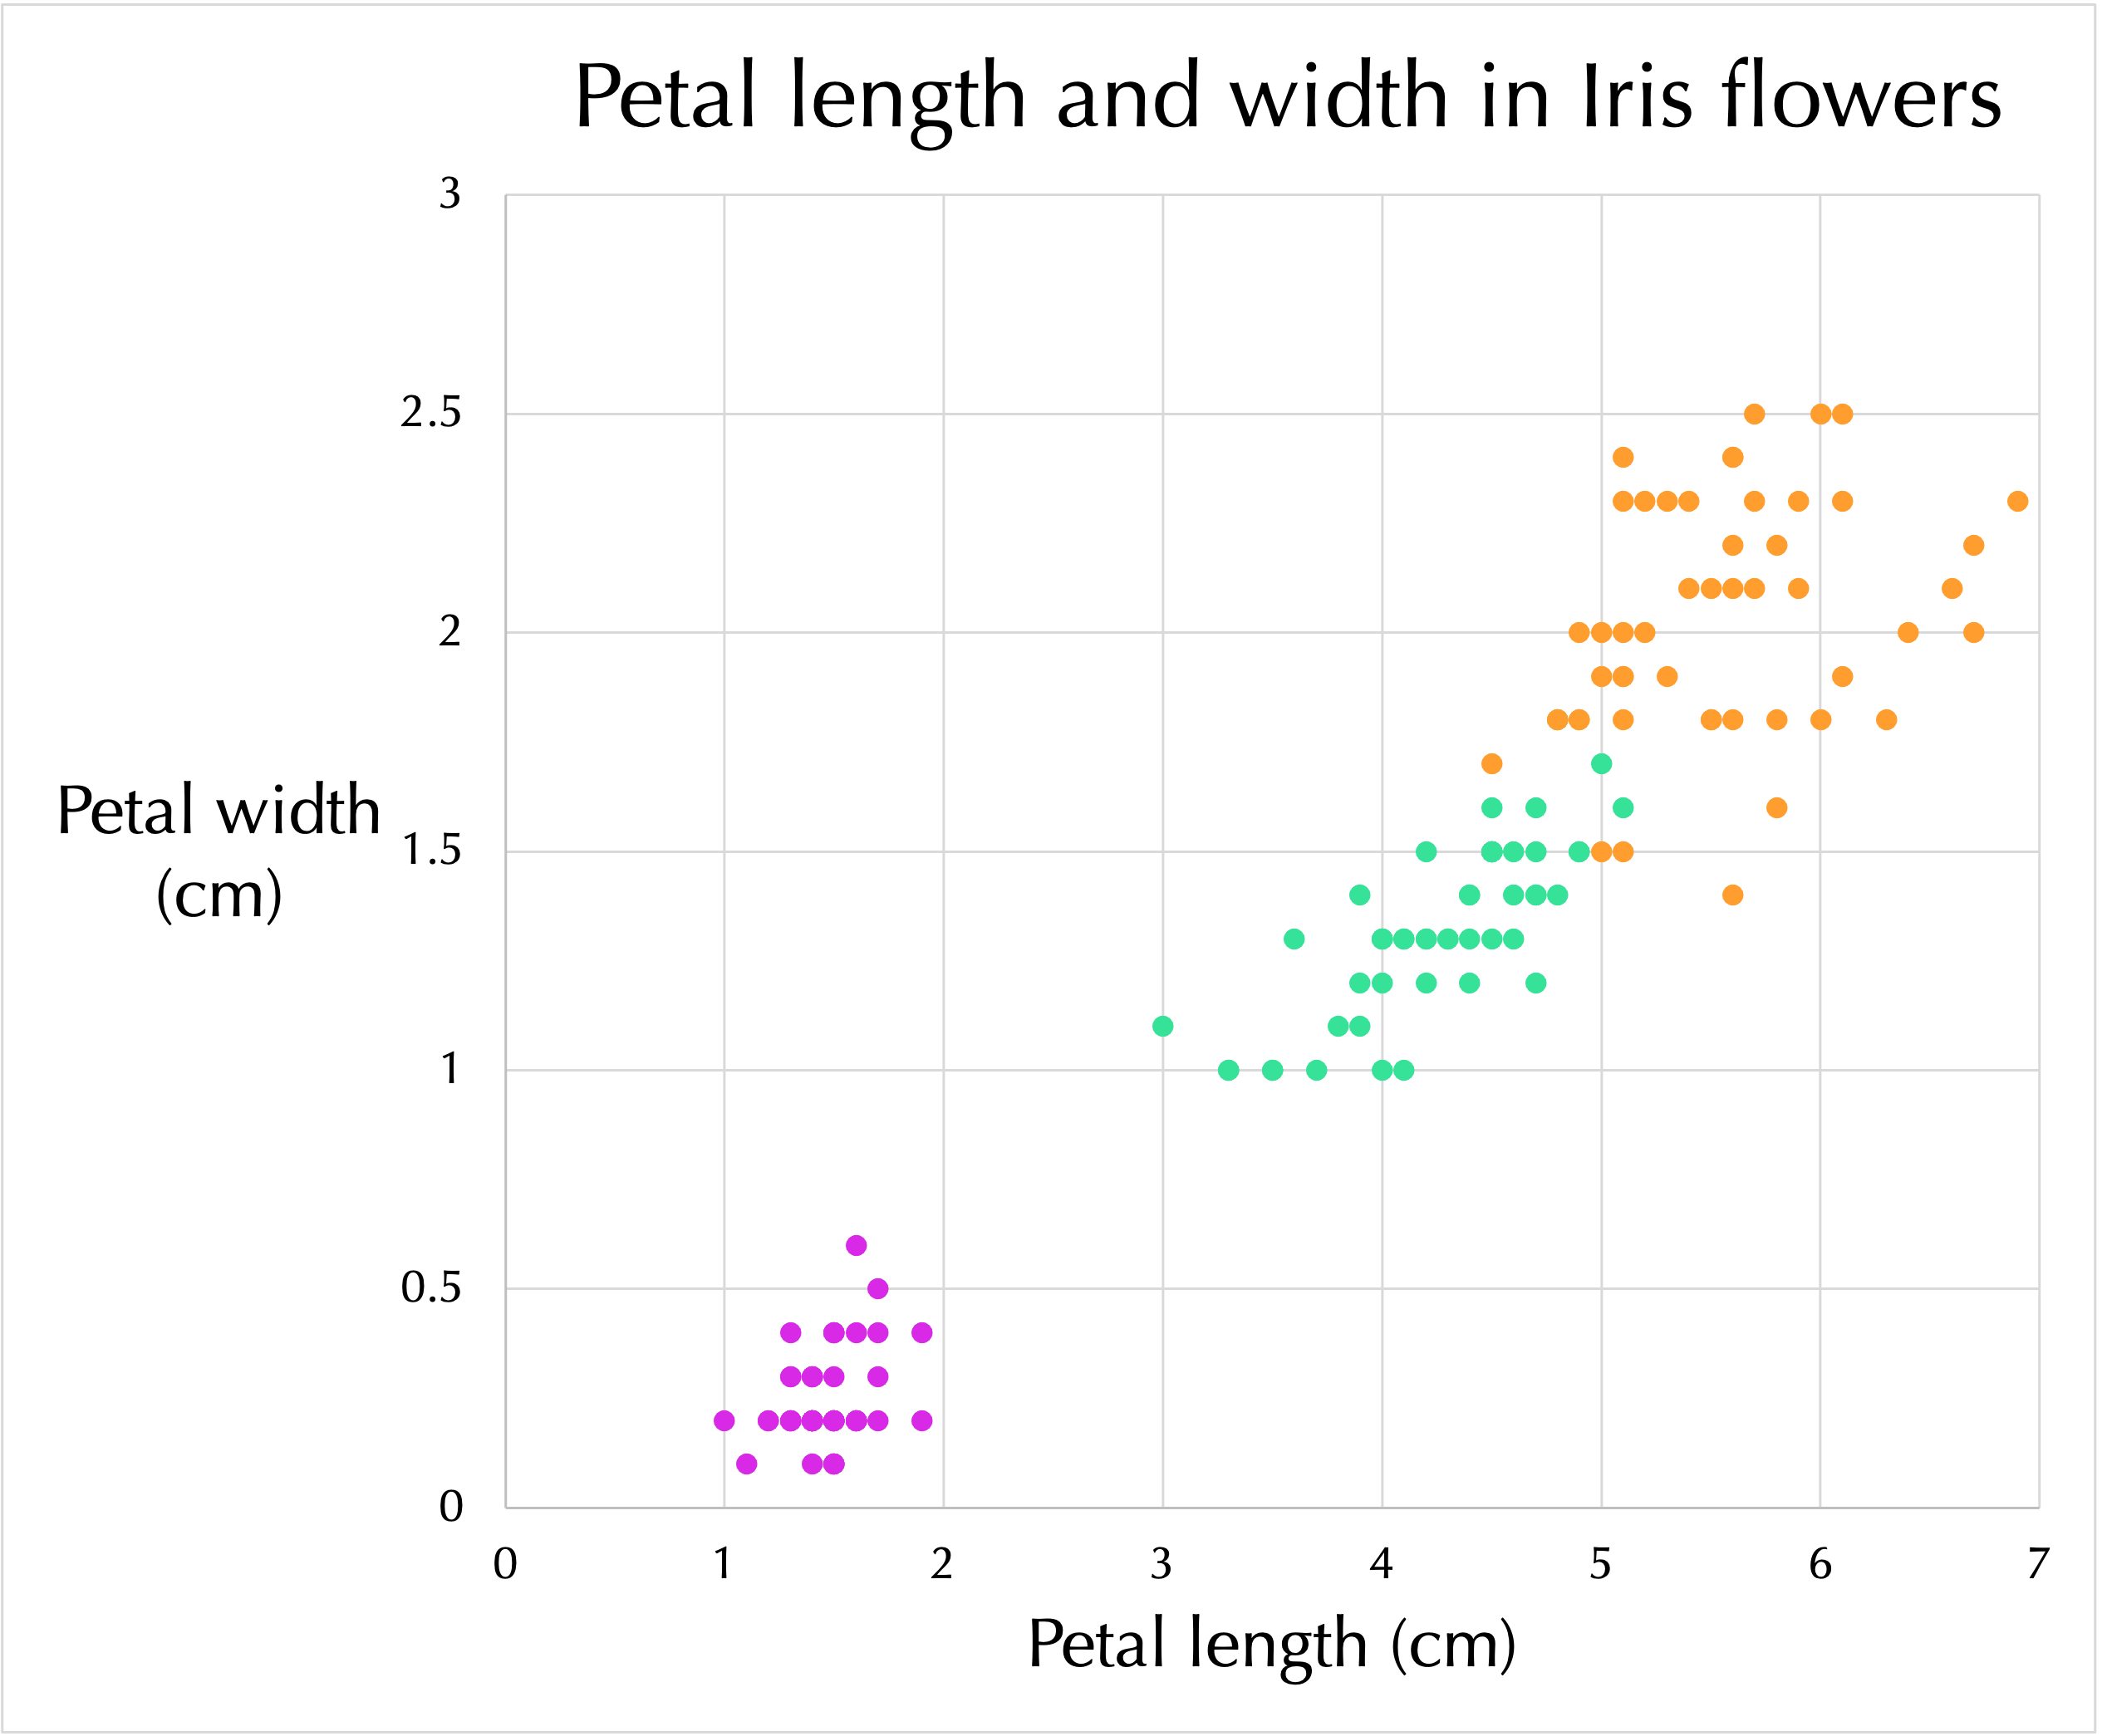
\includegraphics[width = 0.7\textwidth]{../images/iris_petal_data.png}
\caption{Petal width (x-axis) plotted against width (y-axis) for each of the flowers in the iris flower dataset, colored by species. There are not fifty points corresponding to every species because some flowers have the same petal length and width.}
\label{fig:iris_petal_data}
\end{figure}

Note how stark the pattern is in \autoref{fig:iris_petal_data}. Even though we chose only two features from the iris flowers, the points associated with the flowers can be divided into three main clusters by species. In other words, nearby points tend to correspond to flowers from the same species.

If we were to use all four features for the iris dataset, then every flower would be represented by a point in four-dimensional space. For example, the first flower in our initial table of iris features would be represented by the point $(5.1, 3.5, 1.4, 0.2)$. In general, when classifying a collection of data with \textvar{n} features, each element in the dataset can be represented by a \textdefnogloss{feature vector} of length \textvar{n}, whose \textvar{i}-th value corresponds to its value for the \textvar{i}-th feature.

\FloatBarrier
\phantomsection
\subsection{Classifying unknown elements with k-nearest neighbors}

For the iris flower dataset, recall our observation that data points were more likely to belong to the same class if they were nearby. Our hope is that this fact is true for other datasets, that elements from the same class will have feature vectors that are close in \textvar{n}-dimensional space. If so, then we can classify a data point whose class is \textit{unknown} by determining which data points with \textit{known} classification it is near.\\

\begin{qbox}[%
Consider the point with unknown class (gray) in \autoref{fig:knn_neighborhood}. Should it be assigned to the class of the green points or to the class of the blue points?
]\end{qbox}

\begin{figure}[h]
\centering
\mySfFamily
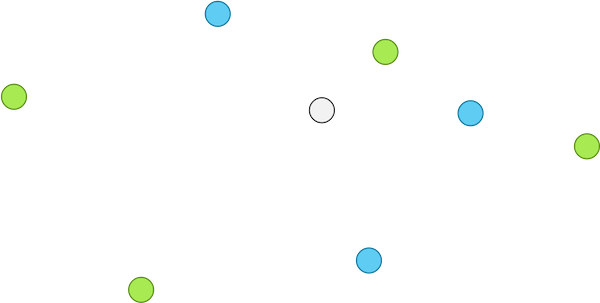
\includegraphics[width = 0.6\textwidth]{../images/knn_neighborhood.png}
\caption{An unknown point (gray) along with a collection of nearby points belonging to two classes, colored green and blue.}
\label{fig:knn_neighborhood}
\end{figure}

The preceding question indicates that classifying points can be surprisingly open-ended. Because of this freedom, researchers have devised a variety of different approaches for classifying data given data with known classes.

We will discuss a simple but powerful classification algorithm called \textdef{k-nearest neighbors (k-NN)}{k-nearest neighbors (k-NN)}{a classification algorithm that assigns each point with unknown class to have the class possessed by the largest number of its \textvar{k} closest neighbors with known class.}. In k-NN, we fix a positive integer \textvar{k} in advance, which will be used for classification of all points. Then, for each point with unknown class, we assign it the class possessed by the largest number of its \textvar{k} closest neighbors.

In the ongoing example, if we were using \textvar{k} equal to 1, then we would assign the unknown point from \autoref{fig:knn_neighborhood} to the green class (\autoref{fig:knn_neighborhood_k=1}).\\

\begin{figure}[h]
\centering
\mySfFamily
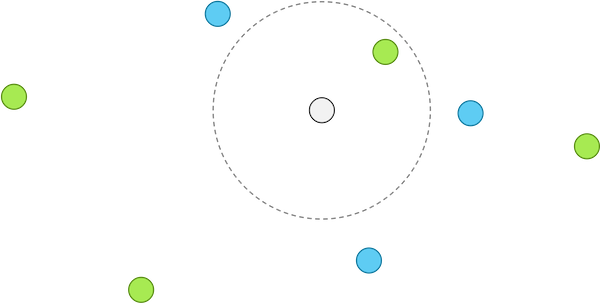
\includegraphics[width = 0.6\textwidth]{../images/knn_neighborhood_k=1.png}
\caption{When using k-NN with \textvar{k} equal to 1, we classify an unknown point according to the point of known class that is nearest; for this reason, the unknown point above would be assigned to the green class.}
\label{fig:knn_neighborhood_k=1}
\end{figure}

However, with the same data and \textvar{k} equal to 4, \autoref{fig:knn_neighborhood_k=4} shows that a majority of the \textvar{k} nearest neighbors are blue, and so we classify the unknown point as blue. This example reinforces a theme of this course, that the results of an algorithm can be sensitive to our choice of parameters.\\

\begin{figure}[h]
\centering
\mySfFamily
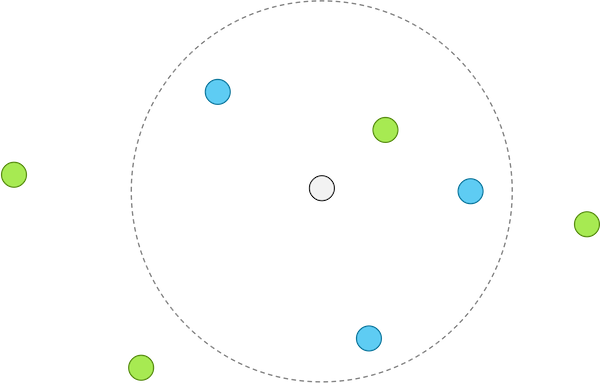
\includegraphics[width = 0.6\textwidth]{../images/knn_neighborhood_k=4.png}
\caption{When using k-NN with \textvar{k} equal to 4, k-NN will classify the unknown point as blue, since three of its four closest neighbors are blue.}
\label{fig:knn_neighborhood_k=4}
\end{figure}

\begin{qbox}[%
When \textvar{k} = 2 or \textvar{k} = 6 for the classification of the point in \autoref{fig:knn_neighborhood}, note that we obtain a tie in the number of points from each known class belonging to the \textvar{k} nearest neighbors of a point with unknown class. How could we break ties in k-NN?
]\end{qbox}

In the more general case in which feature vectors have length \textvar{n}, we can determine which points are nearest to a given point by using the \textdefnogloss{Euclidean distance}, which generalizes the distance between two points in two-dimensional space to vectors in \textvar{n}-dimensional space. Say that we have the vectors $\mathbf{x} = (x_1, x_2, \ldots, x_n)$ and $\mathbf{y} = (y_1, y_2, \ldots, y_n)$. Then the Euclidean distance between them is given by the sum of squares of differences between corresponding vector elements:

$$d(\mathbf{x}, \mathbf{y}) = \sqrt{(x_1 - y_1)^2 + (x_2 - y_2)^2 + \cdots + (x_n-y_n)^2}$$

We now have learned how to use k-NN to classify feature vectors with unknown classes given vectors with known classes. There is just one problem: how can we convert an image of a WBC into a vector?

\FloatBarrier
\phantomsection

\section{Shape Spaces}
\label{sec:shape_spaces}
\phantomsection

\subsection{Interlude: Stone tablets and lost cities}

Imagine that you are a traveler to Earth and come across the ruins of New York City. You find an old road atlas that has driving distances between cities (in miles), shown in \autoref{fig:atlas}. Can you use this atlas to find the other cities? In \autoref{chapter:chemotaxis}, we encountered a ``Lost Immortals'' problem; we call the problem of inferring the locations of cities given the distance between them the ``Lost Cities'' problem.\\

\begin{figure}[h]
\centering
\tabcolsep = 1 em
\mySfFamily
\begin{tabular}{r c c c c c c}
& \textbf{NYC} & \textbf{LA} & \textbf{Pitt.} & \textbf{Miami} & \textbf{Houston} & \textbf{Seattle} \\
\textbf{New York City} & 0 & 2805 & 371 & 1283 & 1628 & 2852 \\
\textbf{Los Angeles} & 2805 & 0 & 2427 & 2733 & 1547 & 1135 \\
\textbf{Pittsburgh} & 371 & 2427 & 0 & 1181 & 1388 & 2502 \\
\textbf{Miami} & 1283 & 2733 & 1181 & 0 & 1189 & 3300 \\
\textbf{Houston} & 1628 & 1547 & 1388 & 1189 & 0 & 2340 \\
\textbf{Seattle} & 2852 & 1135 & 2502 & 3300 & 2340 & 0 \\
\end{tabular}
\caption{All pairwise distances between six cities in the United States.}
\label{fig:atlas}
\end{figure}

\begin{qbox}[%
If you know the location of New York, how could you use the information in the table above to find the other cities?
]\end{qbox}

This seemingly contrived example has a real archaeological counterpart. In 2019, researchers used commercial records that had been engraved by Assyrian merchants onto 19th Century BCE stone tablets in order to estimate distances between pairs of lost Bronze age cities in present-day Turkey. Using this ``atlas'' of sorts, they estimated the locations of the lost cities.

You may be confused as to why biologists should care about stone tablets and lost cities. Let us therefore return to our problem of classifying segmented WBC images by family.

\FloatBarrier
\phantomsection
\subsection{Vectorizing a segmented image}

As we mentioned in the previous section, we would like to apply k-NN to our example of segmented WBC images. Yet k-NN first requires each object to be represented by a feature vector, and so we need some way of converting a WBC image into a feature vector. In this way, we can produce a \textdef{shape space}{shape space}{an assignment of shapes to points in multi-dimensional space}, or an assignment of (cellular image) shapes to points in multi-dimensional space.

You may notice that the problem of ``vectorizing'' a WBC image is similar to one that we have already encountered in \autoref{chapter:coronavirus_1}, when we vectorized a protein structure as the collection of locations of its alpha carbons. Given a protein structure \textvar{S}, we sampled the \textvar{n} alpha carbons from \textvar{S}, producing a vector $\mathbf{s} = (s_1, \ldots, s_n)$, where $s_i$ is the position of the \textvar{i}-th alpha carbon of \textvar{S}.

We will apply the same idea to vectorize our segmented WBCs. Given a binarized image, we will first center the image so that its center of mass is at the origin, and then sample \textvar{n} points from the boundary of the cell nucleus to produce a \textdef{shape vector}{shape vector}{a feature vector for a shape whose features are points on the boundary of the shape} $s = (s_1, \ldots, s_n)$, where $s_i$ is a point with coordinates $(x(i), y(i))$.\\

\begin{note}[%
Both isolating the boundary of a binarized image, and sampling points from this boundary to ensure that points are similarly spaced, are challenging tasks that are outside the scope of our work here, and which we will let CellOrganizer handle for us.
]\end{note}

The feature vector of a binarized image has $2n$ elements, two corresponding to each of the coordinates of its \textvar{n} sampled points. However, it will be more intuitive to think of the shape vector as having length \textvar{n}, with each element having two coordinates.

Furthermore, to determine the ``distance'' between two images' shape vectors, we will use our old friend root mean square deviation (RMSD), which is very similar to the Euclidean distance. Given shape vectors $\mathbf{s}$ and $\mathbf{t}$, the RMSD between these vectors is

$$\text{RMSD}(\mathbf{s}, \mathbf{t}) = \sqrt{\dfrac{1}{n} \cdot (d(s_1, t_1)^2 + d(s_2, t_2)^2 + \cdots + d(s_n, t_n)^2)}\,. $$

\FloatBarrier
\phantomsection
\subsection{Ensuring that image vectorization preserves (dis)similarity}

It is tempting to take the vectorization of every shape as our desired shape space. If this were the case, then we would hope that images of similarly shaped nuclei will have low RMSD and that the more dissimilar two nuclei become, the higher the RMSD of their shape vectors. The potential issues with this assumption are the same as those encountered when discussing protein structures, which we now review.

On the one hand, we need to ensure that the number of points that we sample from the object boundary is sufficiently high to avoid dissimilar shapes from having low RMSD. For this reason, CellOrganizer samples $n = 1000$ points by default for cell nuclei.

On the other hand, we could have very similar shapes whose RMSD winds up being high. For example, recall the shapes in the figure below, which are identical, but one has been flipped and rotated. If we were to vectorize these shapes as they are now in the same way (say, by starting at the top of the shape and proceeding clockwise), then we would obtain two vectors with high RMSD.

REPLACE THIS WITH A LINK TO PREVIOUS IMAGE

We handled this issue in our work on protein structure comparison by introducing the Kabsch algorithm, which identified the best rotation of one shape into another that would minimize the RMSD of the resulting vectors. And yet what makes our work here more complicated is that we are not comparing just two shape vectors in our example of WBC images, we are comparing hundreds.

\FloatBarrier
\phantomsection
\subsection{Inferring a shape space from pairwise distances}

One way to build a shape space for a collection of binarized images is to apply the Kabsch algorithm, which includes a step in which the best rotation is found, to every pair of images. As a result, we would obtain the RMSD between every pair of images, and we would then need to build a shape space from all these distances between pairs of shapes.\\

\begin{note}[%
CellOrganizer has one applies an alternative approach to the Kabsch algorithm for computing a cellular distance, called the \textdefnogloss{diffeomorphic distance}, which can be thought of intuitively as determining the amount of energy required to deform one shape into another.
]\end{note}

We hope that this problem sounds familiar, as it is the Lost Cities problem in disguise. The pairs of distances between images correspond to a road atlas, and placing images into a shape space corresponds to locating cities.

Statisticians have devised a collection of approaches to solve the Lost Cities problem, the most common of which are called multi-dimensional scaling. The fundamental idea of multi-dimensional scaling is to assign points to \textvar{n}-dimensional space such that the distances between points in this space approximately resemble a collection of distances between pairs of objects in some dataset (which in our case is cellular images).\\

\begin{qbox}[%
If we have \textvar{m} cellular images, then how many times will we need to compute the distance between a pair of images?
]\end{qbox}

\FloatBarrier
\phantomsection
\subsection{Aligning many images concurrently}

Unfortunately, if we have a large dataset, then computing the distance between every pair of objects can become very time-intensive, even with a powerful computer. Instead, we will rotate all images \textit{concurrently}. After this alignment, we can then center and vectorize all the images starting at the same position.

One way of aligning a collection of images is to first identify the \textdef{major axis}{major axis}{the line segment crossing through an object's center of mass that is as long as possible} of each image, which is the line segment crossing through the image's center of mass that is as long as possible. \autoref{fig:three_similar_shapes_unaligned} shows the major axis for a few shapes that may not immediately look similar.

\begin{figure}[h]
\centering
\mySfFamily
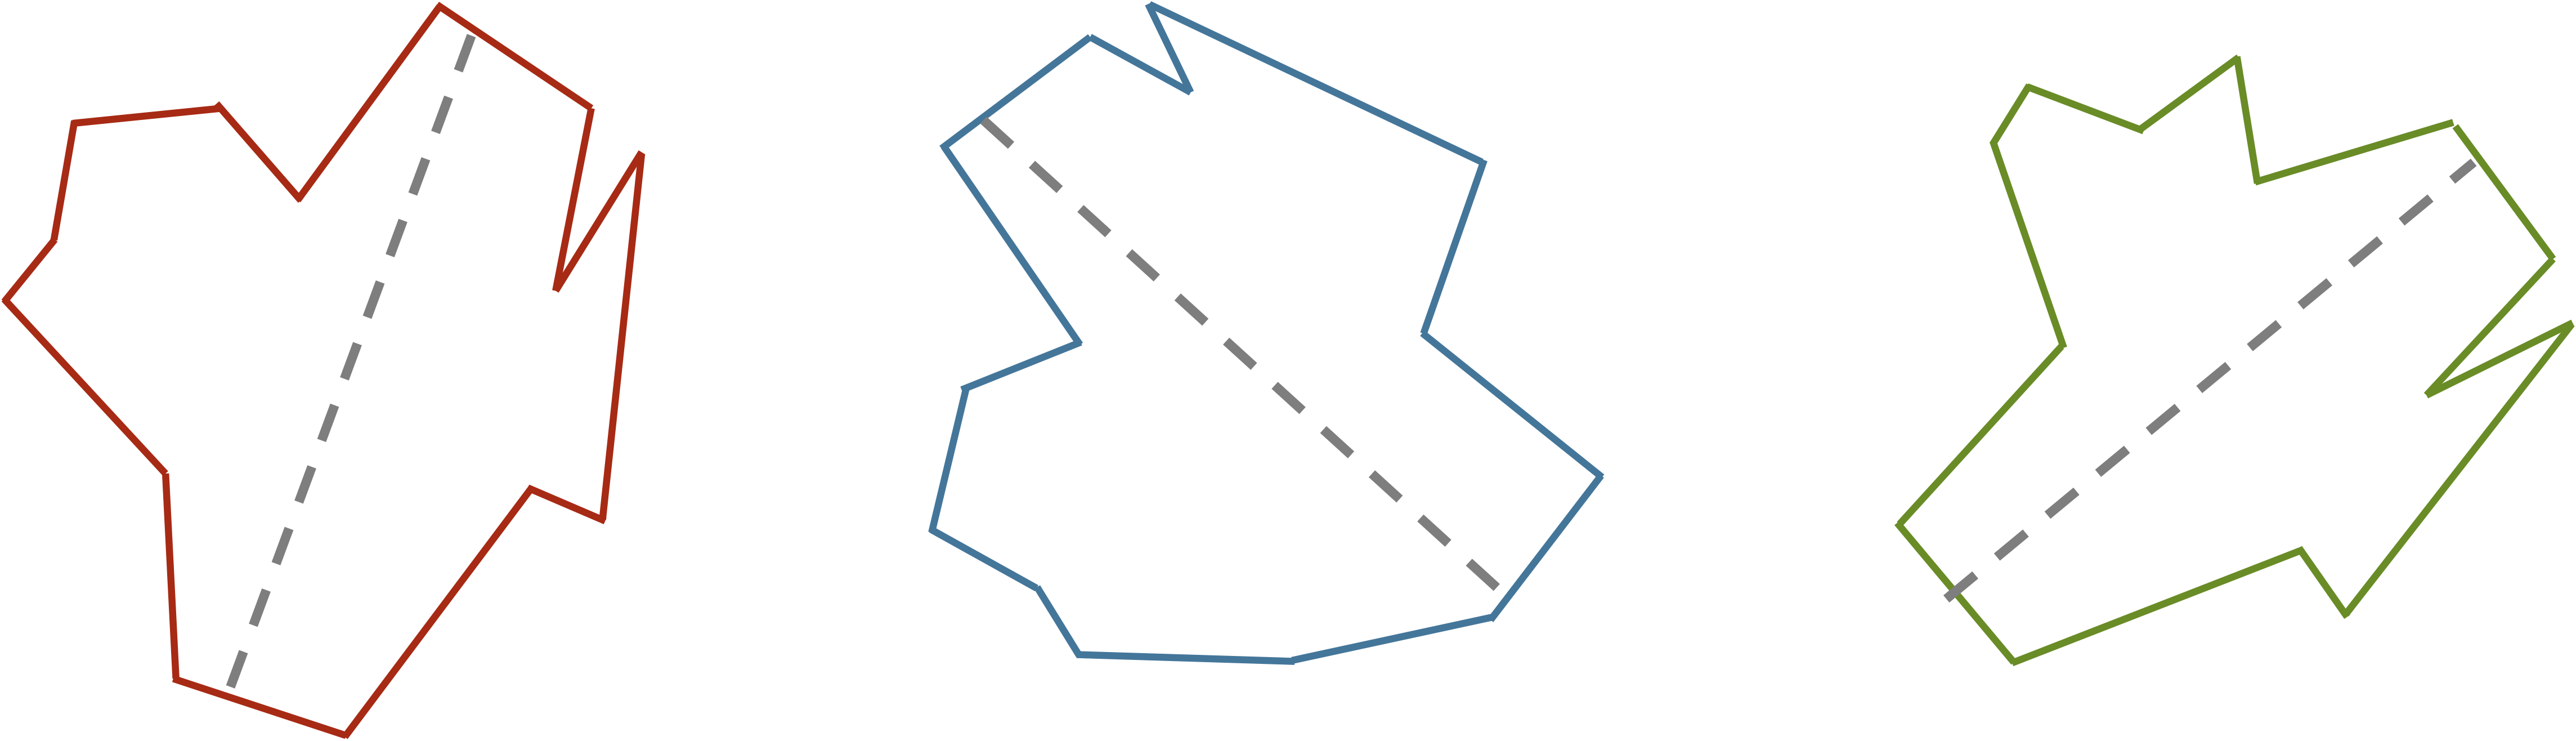
\includegraphics[width = 0.8\textwidth]{../images/three_similar_shapes_unaligned.png}
\caption{Three similar shapes, with their major axes highlighted in gray.}
\label{fig:three_similar_shapes_unaligned}
\end{figure}

When we align the major axes of similar shapes, their similarities will overlap (\autoref{fig:three_similar_shapes_aligned}). These images are ready to be vectorized (say, starting from the point on the right side of an image's major axis and proceeding counterclockwise). The resulting vectors will have low RMSD because corresponding points on the shapes will be nearby.

\begin{figure}[h]
\centering
\mySfFamily
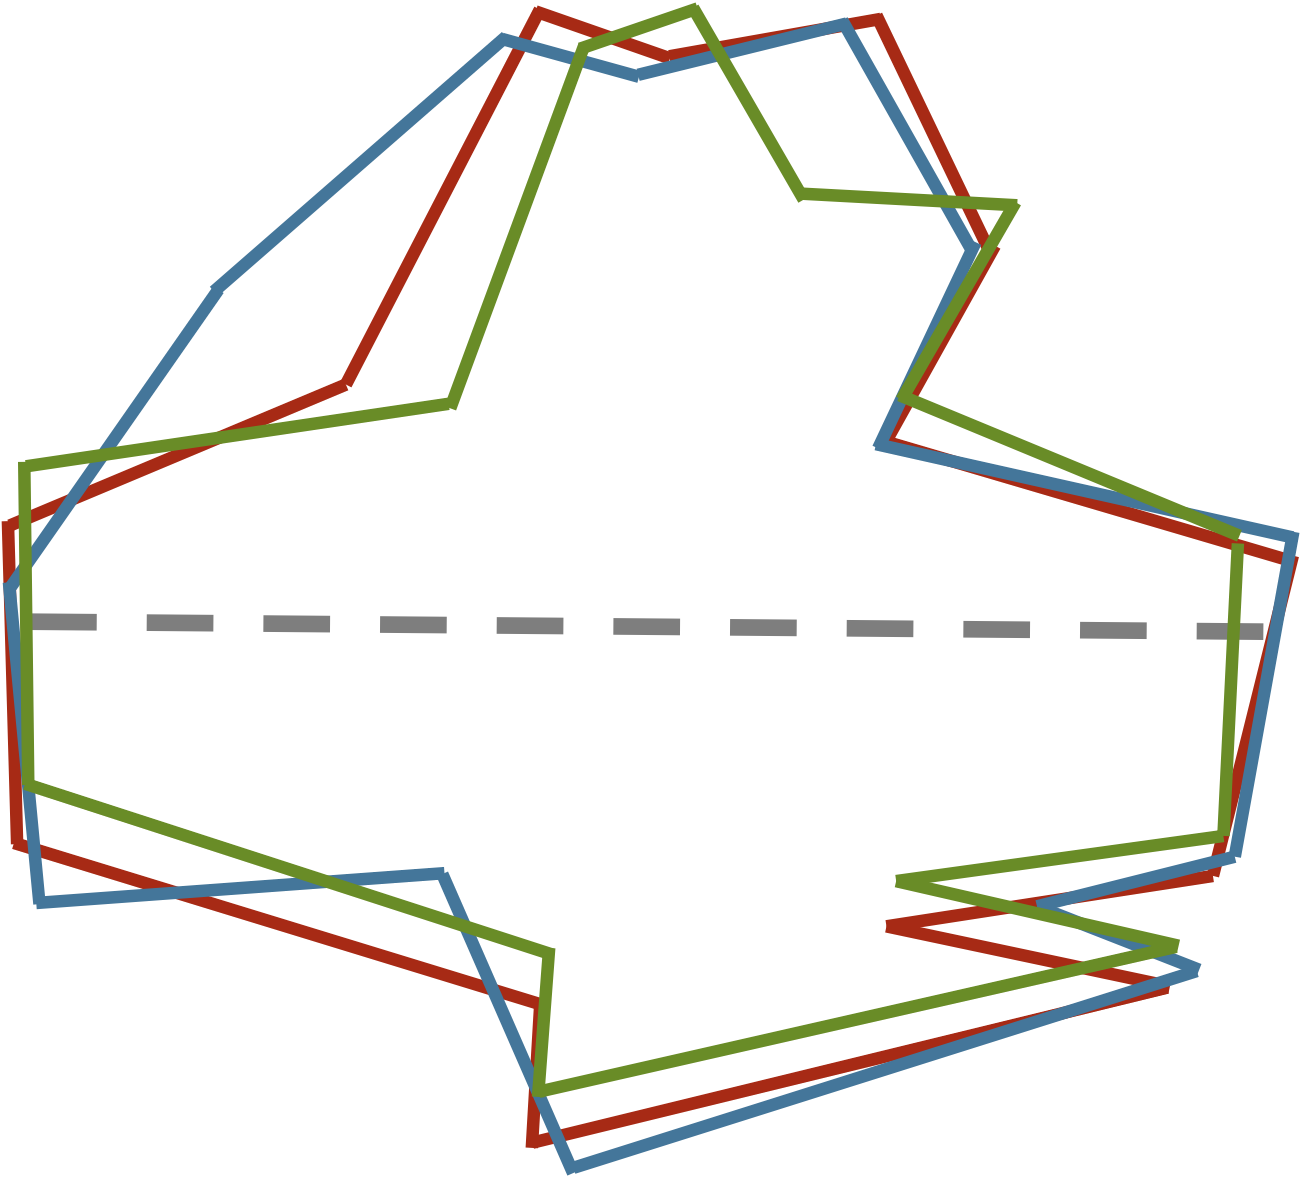
\includegraphics[width = 0.4\textwidth]{../images/three_similar_shapes_aligned.png}
\caption{Aligning the three images from \autoref{fig:three_similar_shapes_unaligned} so that their major axes overlap allows us to see similarities between the shapes as well as build consistent shape vectors for them.}
\label{fig:three_similar_shapes_aligned}
\end{figure}

\begin{note}[%
When we align images along their major axes, we need to ensure that a shape's mirror image is not a better alignment. Handling this issue is beyond the scope of our work here but is discussed in the literature.
]\end{note}

By vectorizing a collection of binarized cellular images after alignment, the resulting vectors form our desired shape space. To review, each vector correspond to a sampling of \textvar{n} points from the boundary of each image, which can be translated into a vector of $2n$ coordinates. Yet one more pitfall remains.


\FloatBarrier
\phantomsection

\section{Principal Components Analysis}
\label{sec:pca}

\phantomsection
\subsection{The curse of dimensionality}

Things get weird in multi-dimensional space.

Consider a circle inscribed in a square, as shown in \autoref{fig:inscribed_circle_and_sphere}. The ratio of the area of the circle to the area of the square is $π/4 \approx 0.785$, regardless of the side length. When we move to three dimensions and have a sphere inscribed in a cube, the ratio of the volume of the sphere to that of the cube is $(4π/3)/8 \approx 0.524$.\\

\begin{figure}[h]
\centering
\mySfFamily
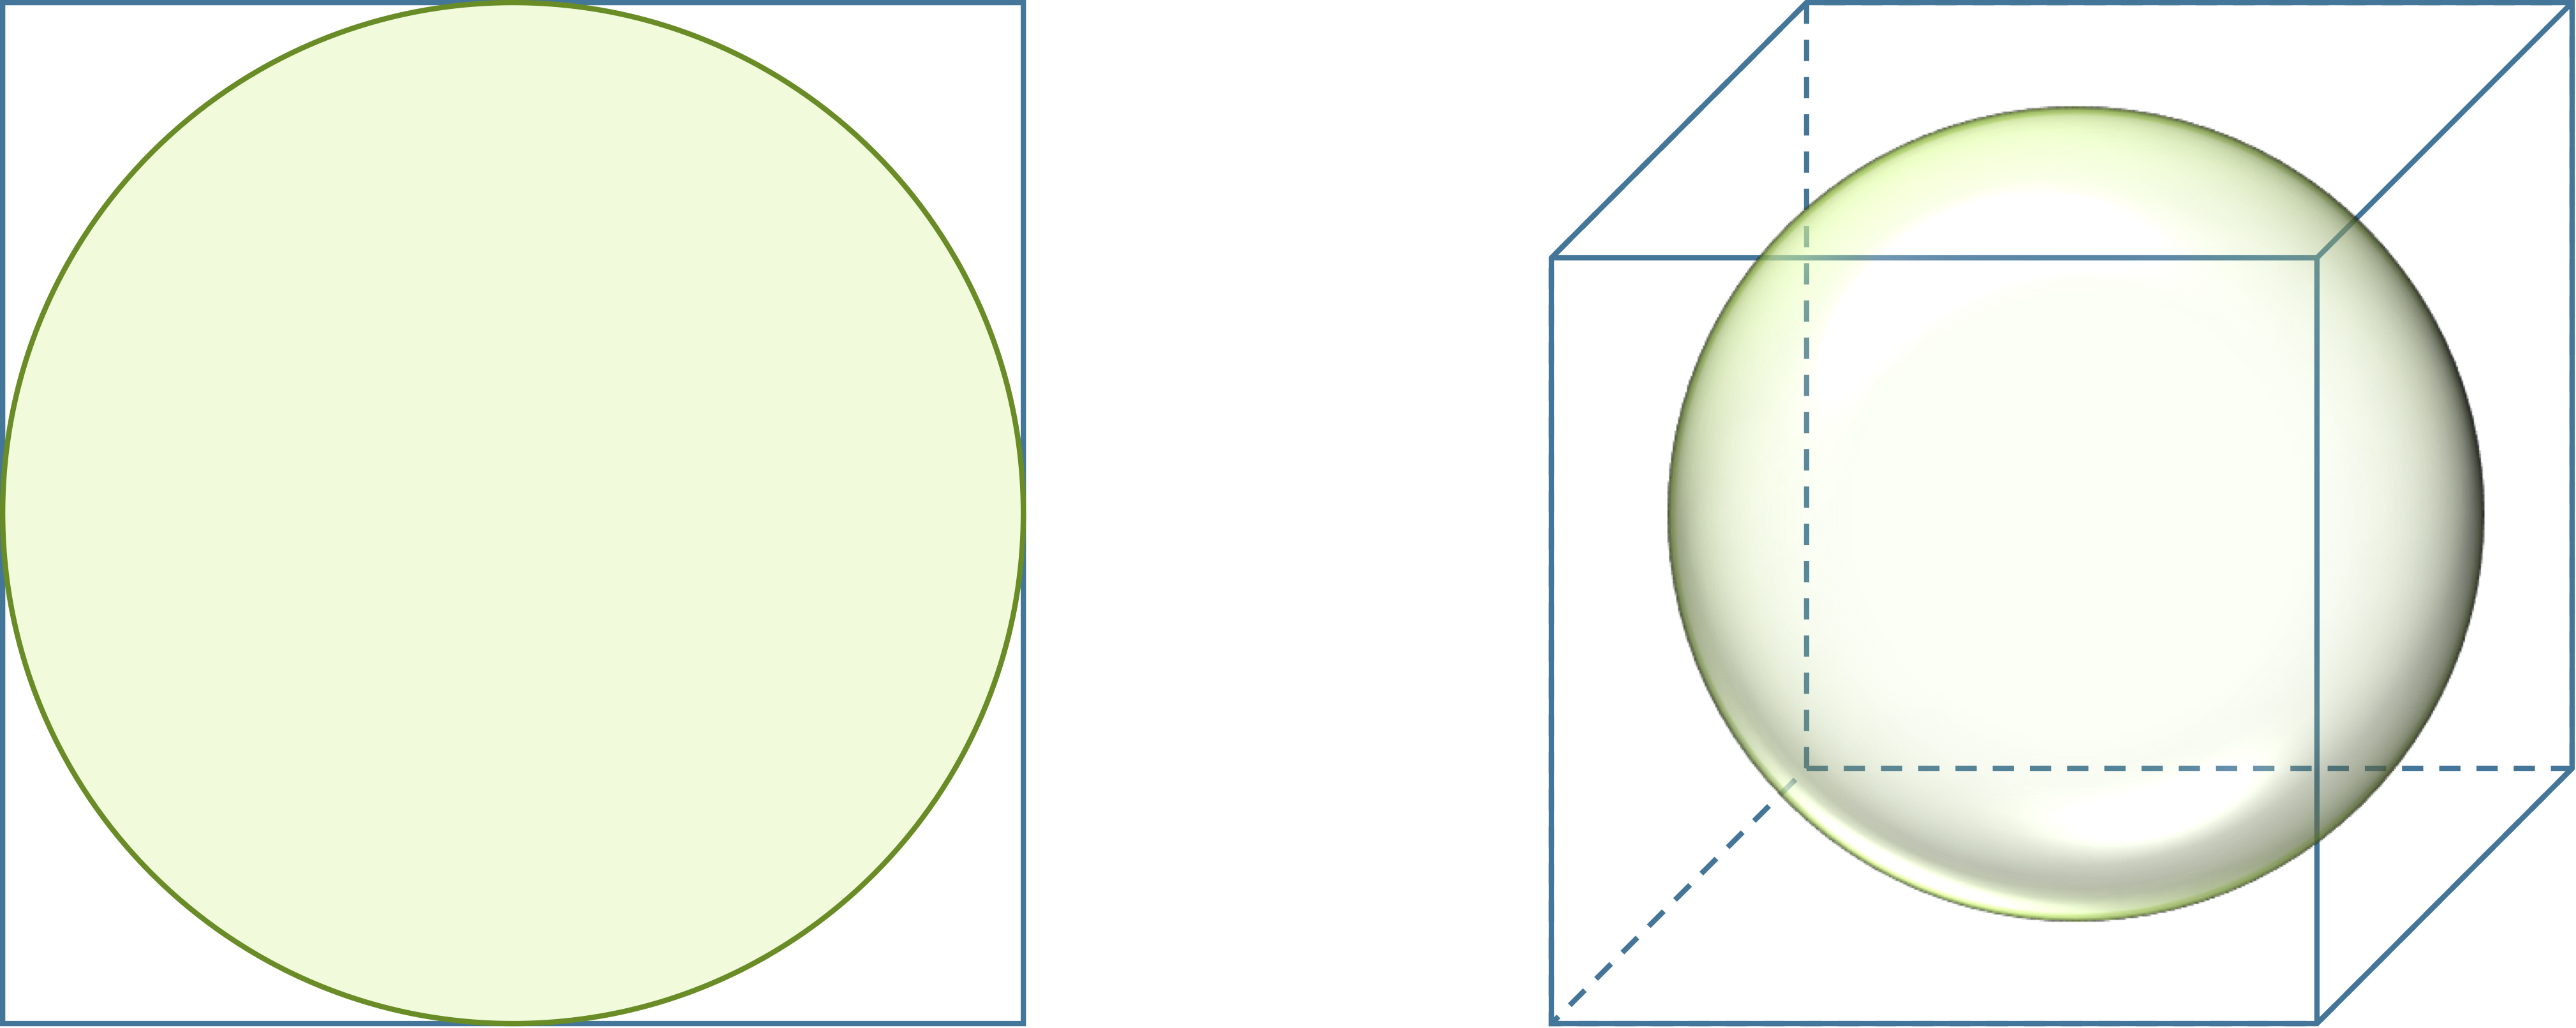
\includegraphics[width = 0.8\textwidth]{../images/inscribed_circle_and_sphere.png}
\caption{A circle inscribed in a square takes up more of the square (78.5 percent) than a sphere inscribed in a cube (52.4 percent).}
\label{fig:inscribed_circle_and_sphere}
\end{figure}

We define an \textvar{n}-dimensional unit sphere as the set of points in \textvar{n}-dimensional space whose (Euclidean) distance from the origin is at most 1, and an \textvar{n}-dimensional cube as the set of points whose coordinates are all between 0 and 1. A precise definition of the volume of a multi-dimensional object is beyond the scope of our work, but as \textvar{n} increases, the sphere takes up less and less of the cube. As \textvar{n} tends toward infinity, the ratio of the volume of the \textvar{n}-dimensional unit sphere to the volume of the \textvar{n}-dimensional unit cube approaches zero!

One way of interpreting the vanishing of the sphere's volume is that the cube has more corners than a square does, and so the more dimensions that we have, the more corners in which there are to hide away from the sphere. In other words, as we increase the number of dimensions, most of the volume of an object winds up scattering outward from the object's center.

The vanishing sphere seem like an arcane triviality holding interest only for mathematicians toiling in fluorescently lit academic offices at strange hours. Yet this little story is just one manifestation of a very deep paradigm in data science called the \textdef{curse of dimensionality}{curse of dimensionality}{a collection of principles that arise in higher dimensions that run counter to our intuition about our three-dimensional existence}, a collection of principles that arise in higher dimensions that run counter to our intuition about our three-dimensional existence.

\FloatBarrier
\phantomsection
\subsection{How the curse of dimensionality affects classification}

In the previous section, we discussed sampling \textvar{n} points from the boundary of an image, thus converting the image into a vector in a space with $2n$ dimensions. We argued that \textvar{n} needs to be sufficiently large to ensure that comparing the vectors of two images will give an accurate representation of how similar their shapes are. And yet the size of \textvar{n} means that we need to be careful about the curse of dimensionality.

Say that we sample \textvar{k} points randomly from the interior of an \textvar{n}-dimensional unit hypercube. Let $d_{\text{min}}$ and $d_{\text{max}}$ denote the minimum and maximum distance from any of our points to the origin, respectively. As \textvar{n} grows, the ratio $d_{\text{min}}d_{\text{max}}$ heads toward 1; in other words, the minimum distance between points becomes indistinguishable from the maximum distance between points.

This other facet of the curse of dimensionality means that algorithms like k-NN, which classify points with unknown classes based on nearby points with known classes, may not perform well in higher-dimensional spaces in which even similar points tend to fly away from each other.

Because of the curse of dimensionality, it makes sense to reduce the number of dimensions before performing any further analysis. We could reduce the number of features used for generating a vector, especially if we have reason to believe that some features are more informative than others. This approach will likely not work for our WBC image example, since it is not clear why one point on the boundary of our images would be inherently better than another.

Instead, we will reduce the number of dimensions of our shape space without removing any features from the data. As perplexing as multi-dimensional space may already seem, it may be totally unclear how we could reduce the dimensions of a space. We will therefore explain dimension reduction in the context of three-dimensional space; our approach may be more familiar than you think.

\FloatBarrier
\phantomsection
\subsection{Dimension reduction with principal components analysis}

We will introduce dimension reduction using the iris flower dataset that we introduced when discussing classification. Although this dataset has four features, we will focus again on only petal length and width, which we plot against each other in \autoref{fig:iris_petal_data_unlabeled}. We can trust our eyes to notice the clear pattern: as iris petal width increases, petal length tends to increase as well.

\begin{figure}[h]
\centering
\mySfFamily
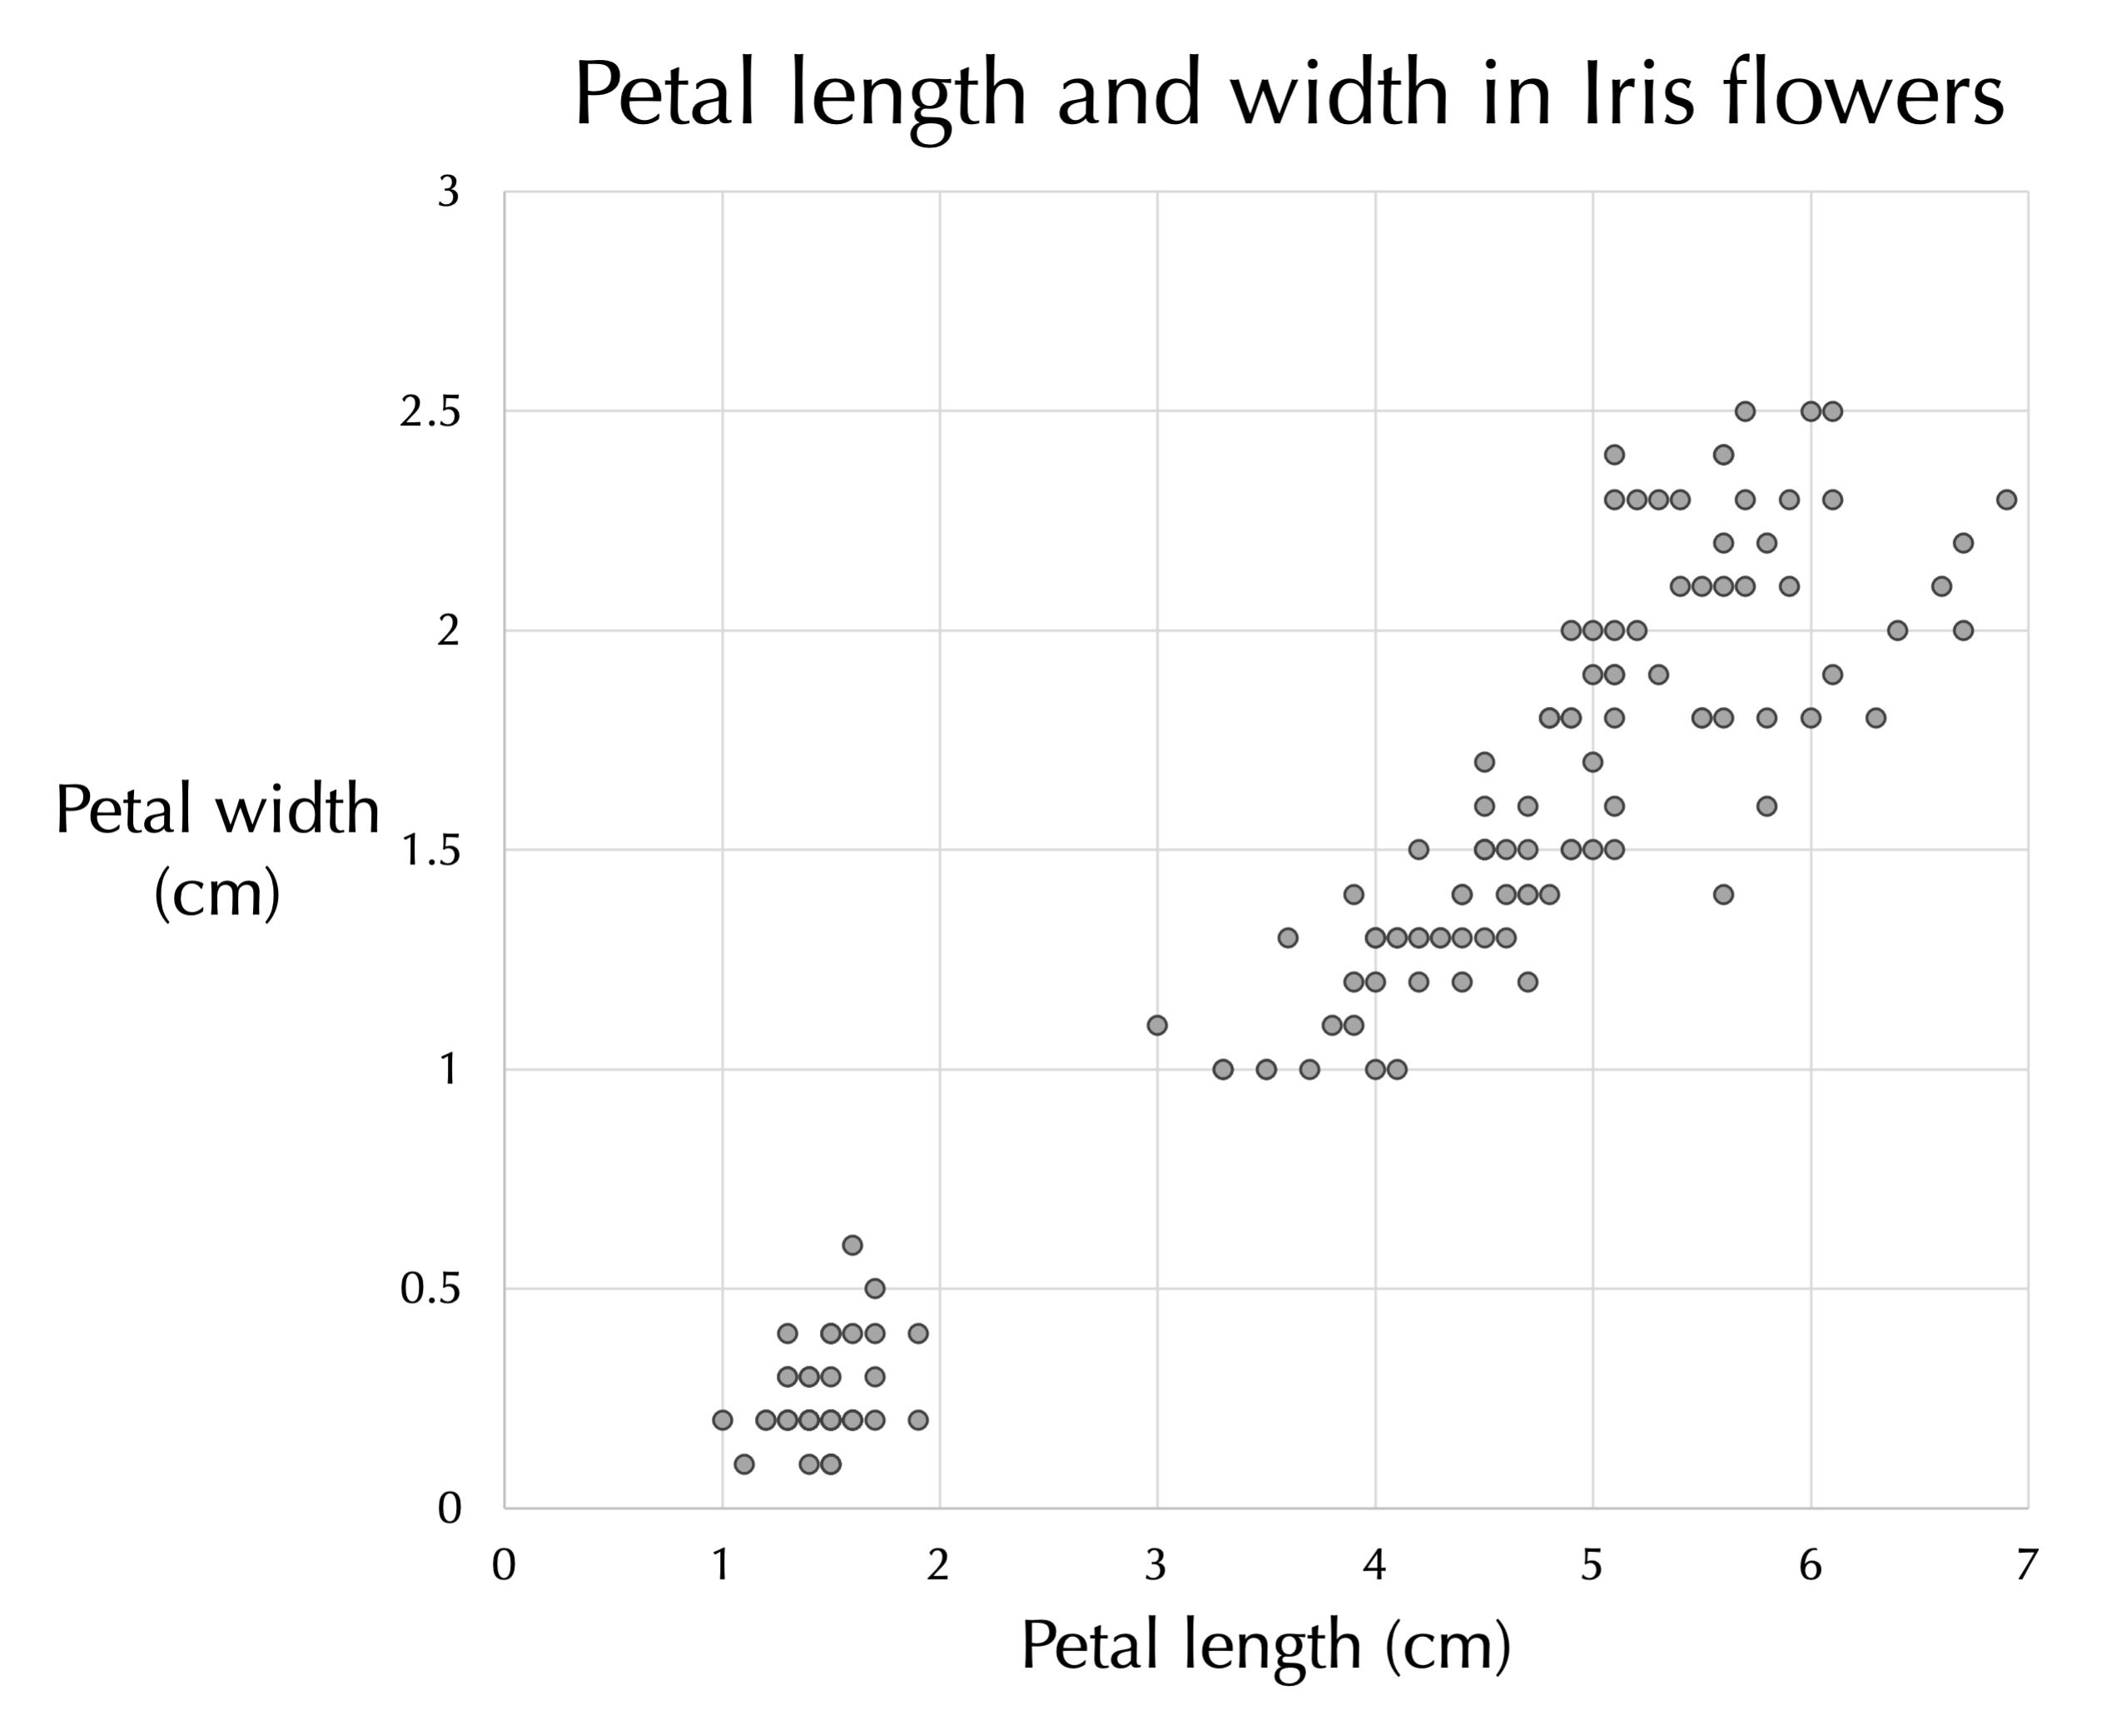
\includegraphics[width = 0.7\textwidth]{../images/iris_petal_data_unlabeled.png}
\caption{Petal width (x-axis) plotted against petal width (y-axis) for all flowers in the iris flower dataset, not labeled according to species.}
\label{fig:iris_petal_data_unlabeled}
\end{figure}

If we draw a line through the center of the data (\autoref{fig:iris_flowers_regression_line}), then the line provides a reasonable estimate of a flower's petal width given its length, and vice-versa. This line, a one-dimensional object, therefore approximates a collection of points in two dimensions.\\

\begin{figure}[h]
\centering
\mySfFamily
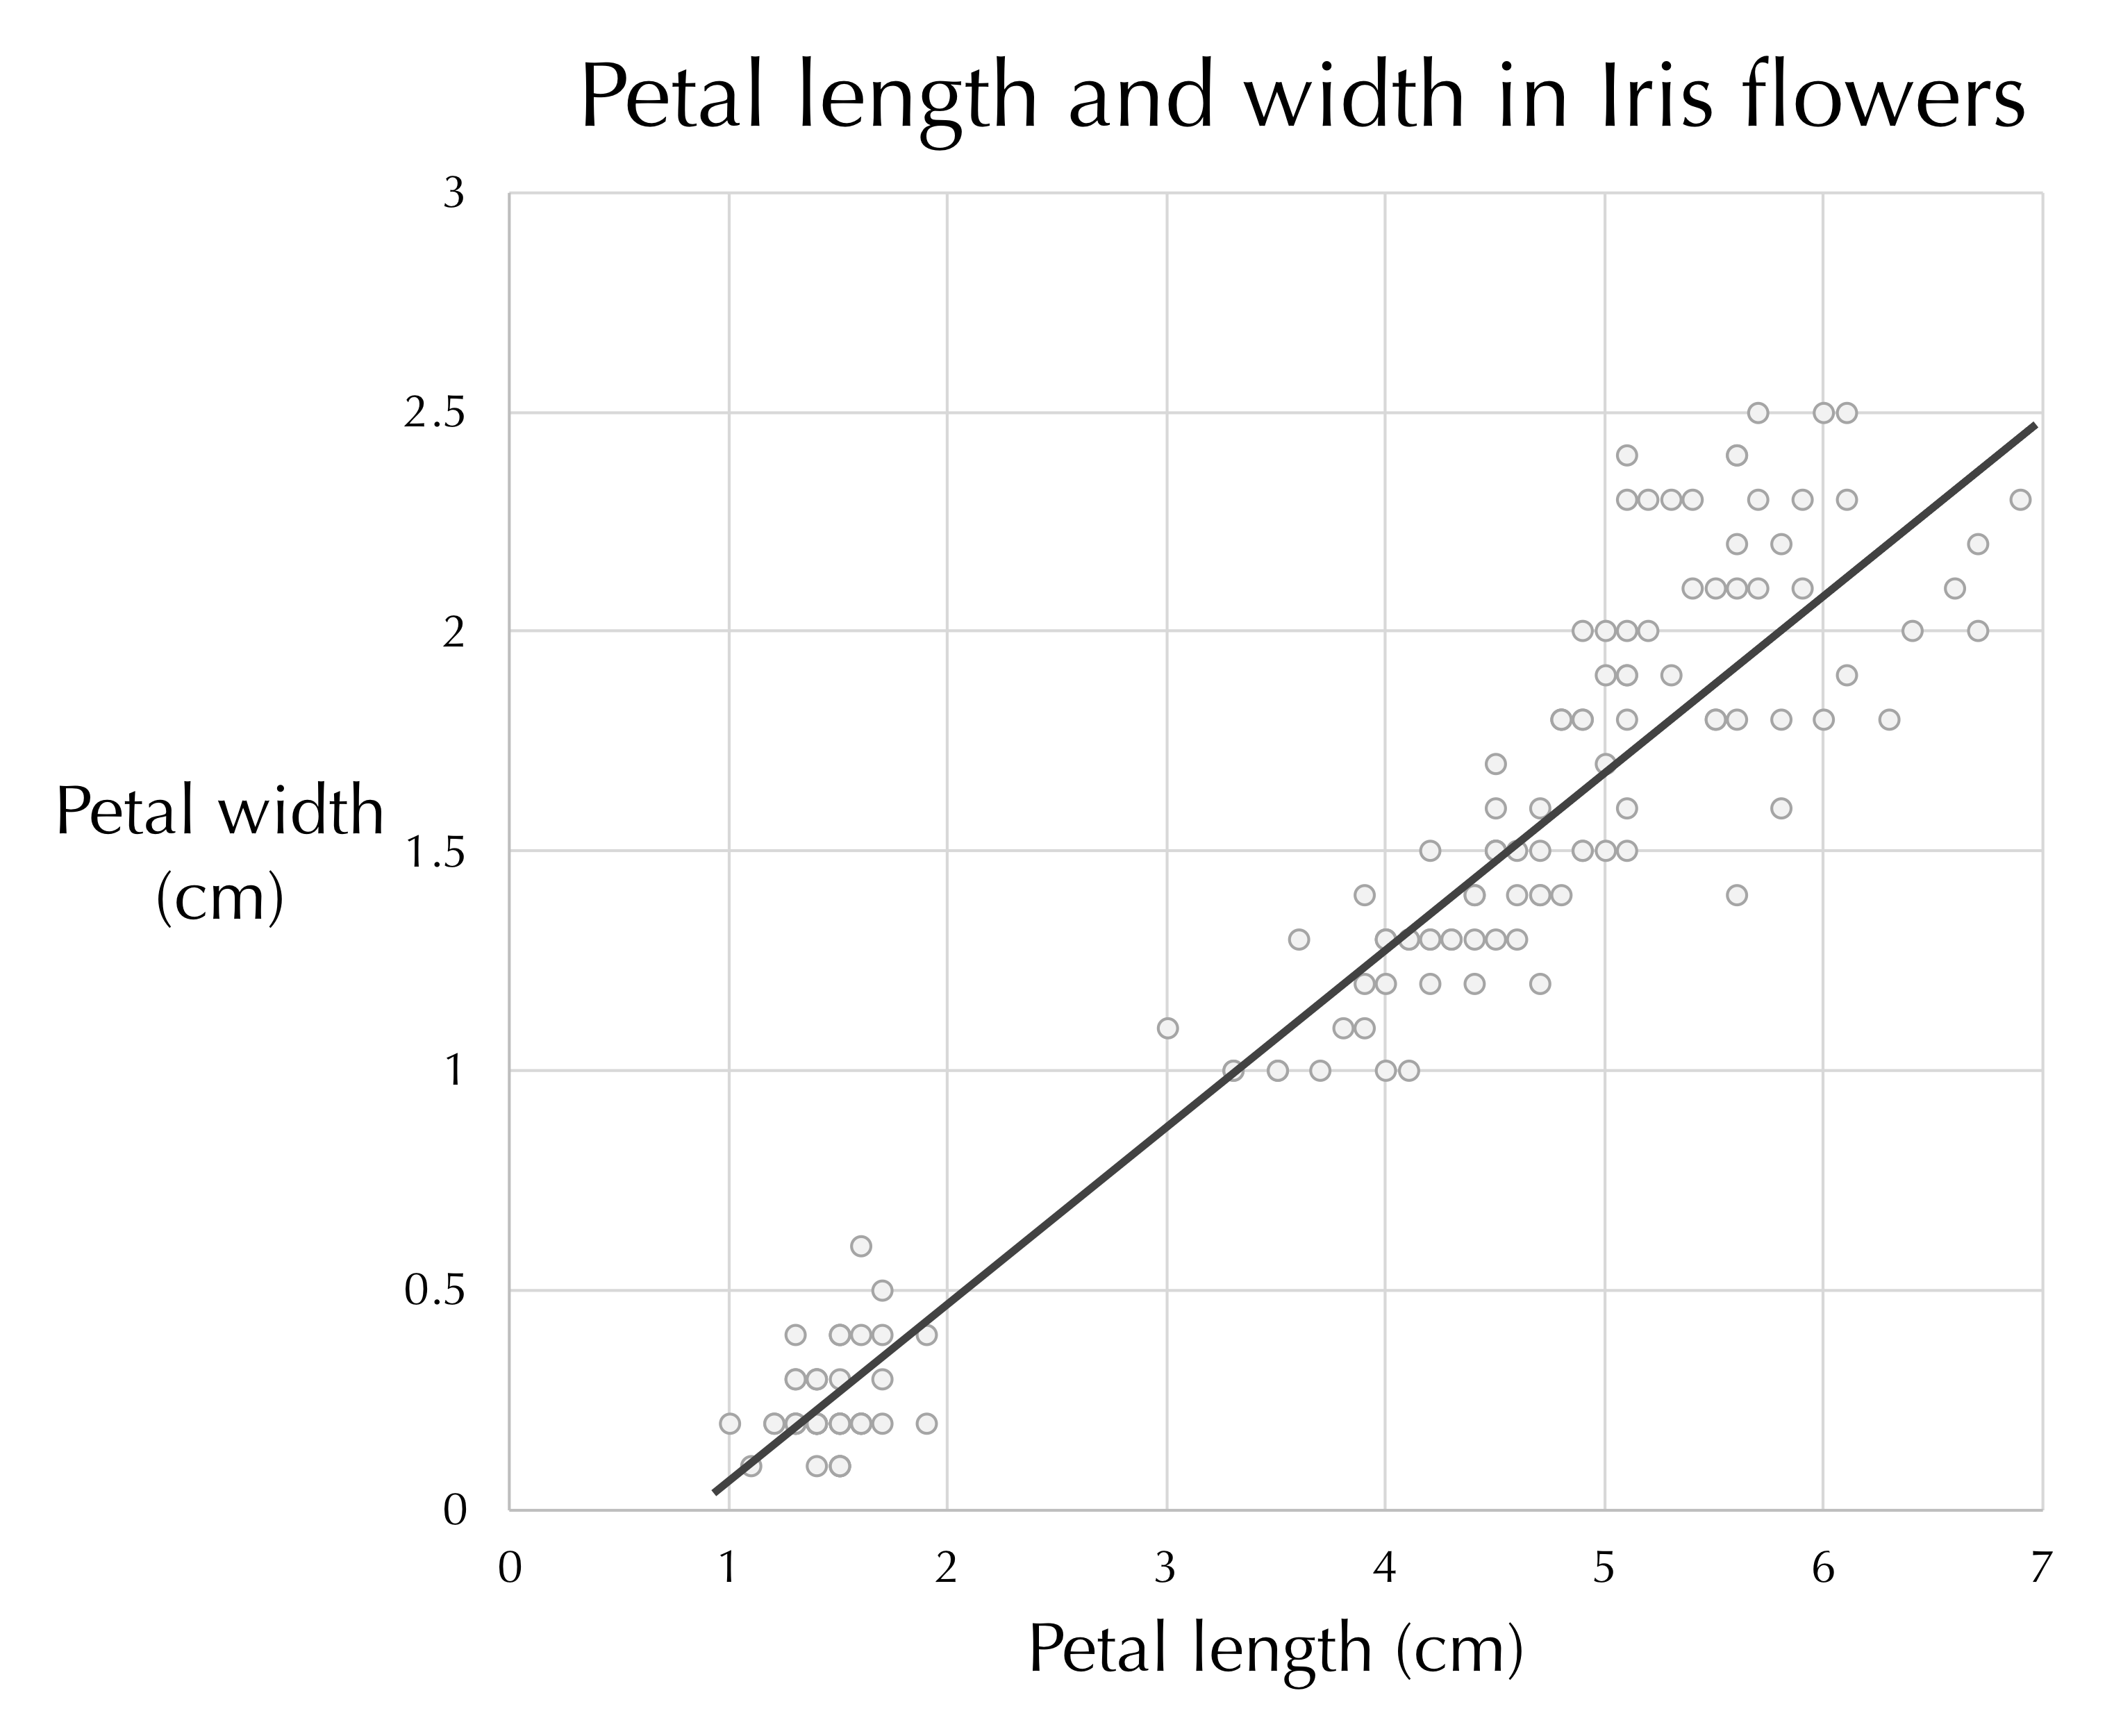
\includegraphics[width = 0.7\textwidth]{../images/iris_flowers_regression_line.png}
\caption{A line passing through the plot of iris petal length against petal width. The line tells us approximately how wide we can expect an iris petal to be given the petal's width, and vice-versa.}
\label{fig:iris_flowers_regression_line}
\end{figure}

\begin{qbox}[%
How could we have determined the line in \autoref{fig:iris_flowers_regression_line}?
]\end{qbox}

Long ago in math class, you may have learned how to choose a line to best approximate a two-dimensional dataset using \textdefnogloss{linear regression}, which we will now briefly describe. In regression, we first establish one variable as the \textit{dependent} variable, which is typically plotted on the y-axis. In our iris flower example, the dependent variable is petal width.

Given a line, we use $L(x)$ to denote the y-coordinate of the point on the line corresponding to a given x-coordinate. For this line, we can then define the \textdefnogloss{residual} of a data point $(x, y)$ as the difference $y - L(x)$ between its y-coordinate and the y-coordinate that the line estimates as corresponding to \textvar{x}. If a residual is positive, then the data point lies ``above'' the line, and if the residual is negative, then the point lies ``below'' the line (\autoref{fig:residuals_y_coordinates}).\\

\begin{figure}[h]
\centering
\mySfFamily
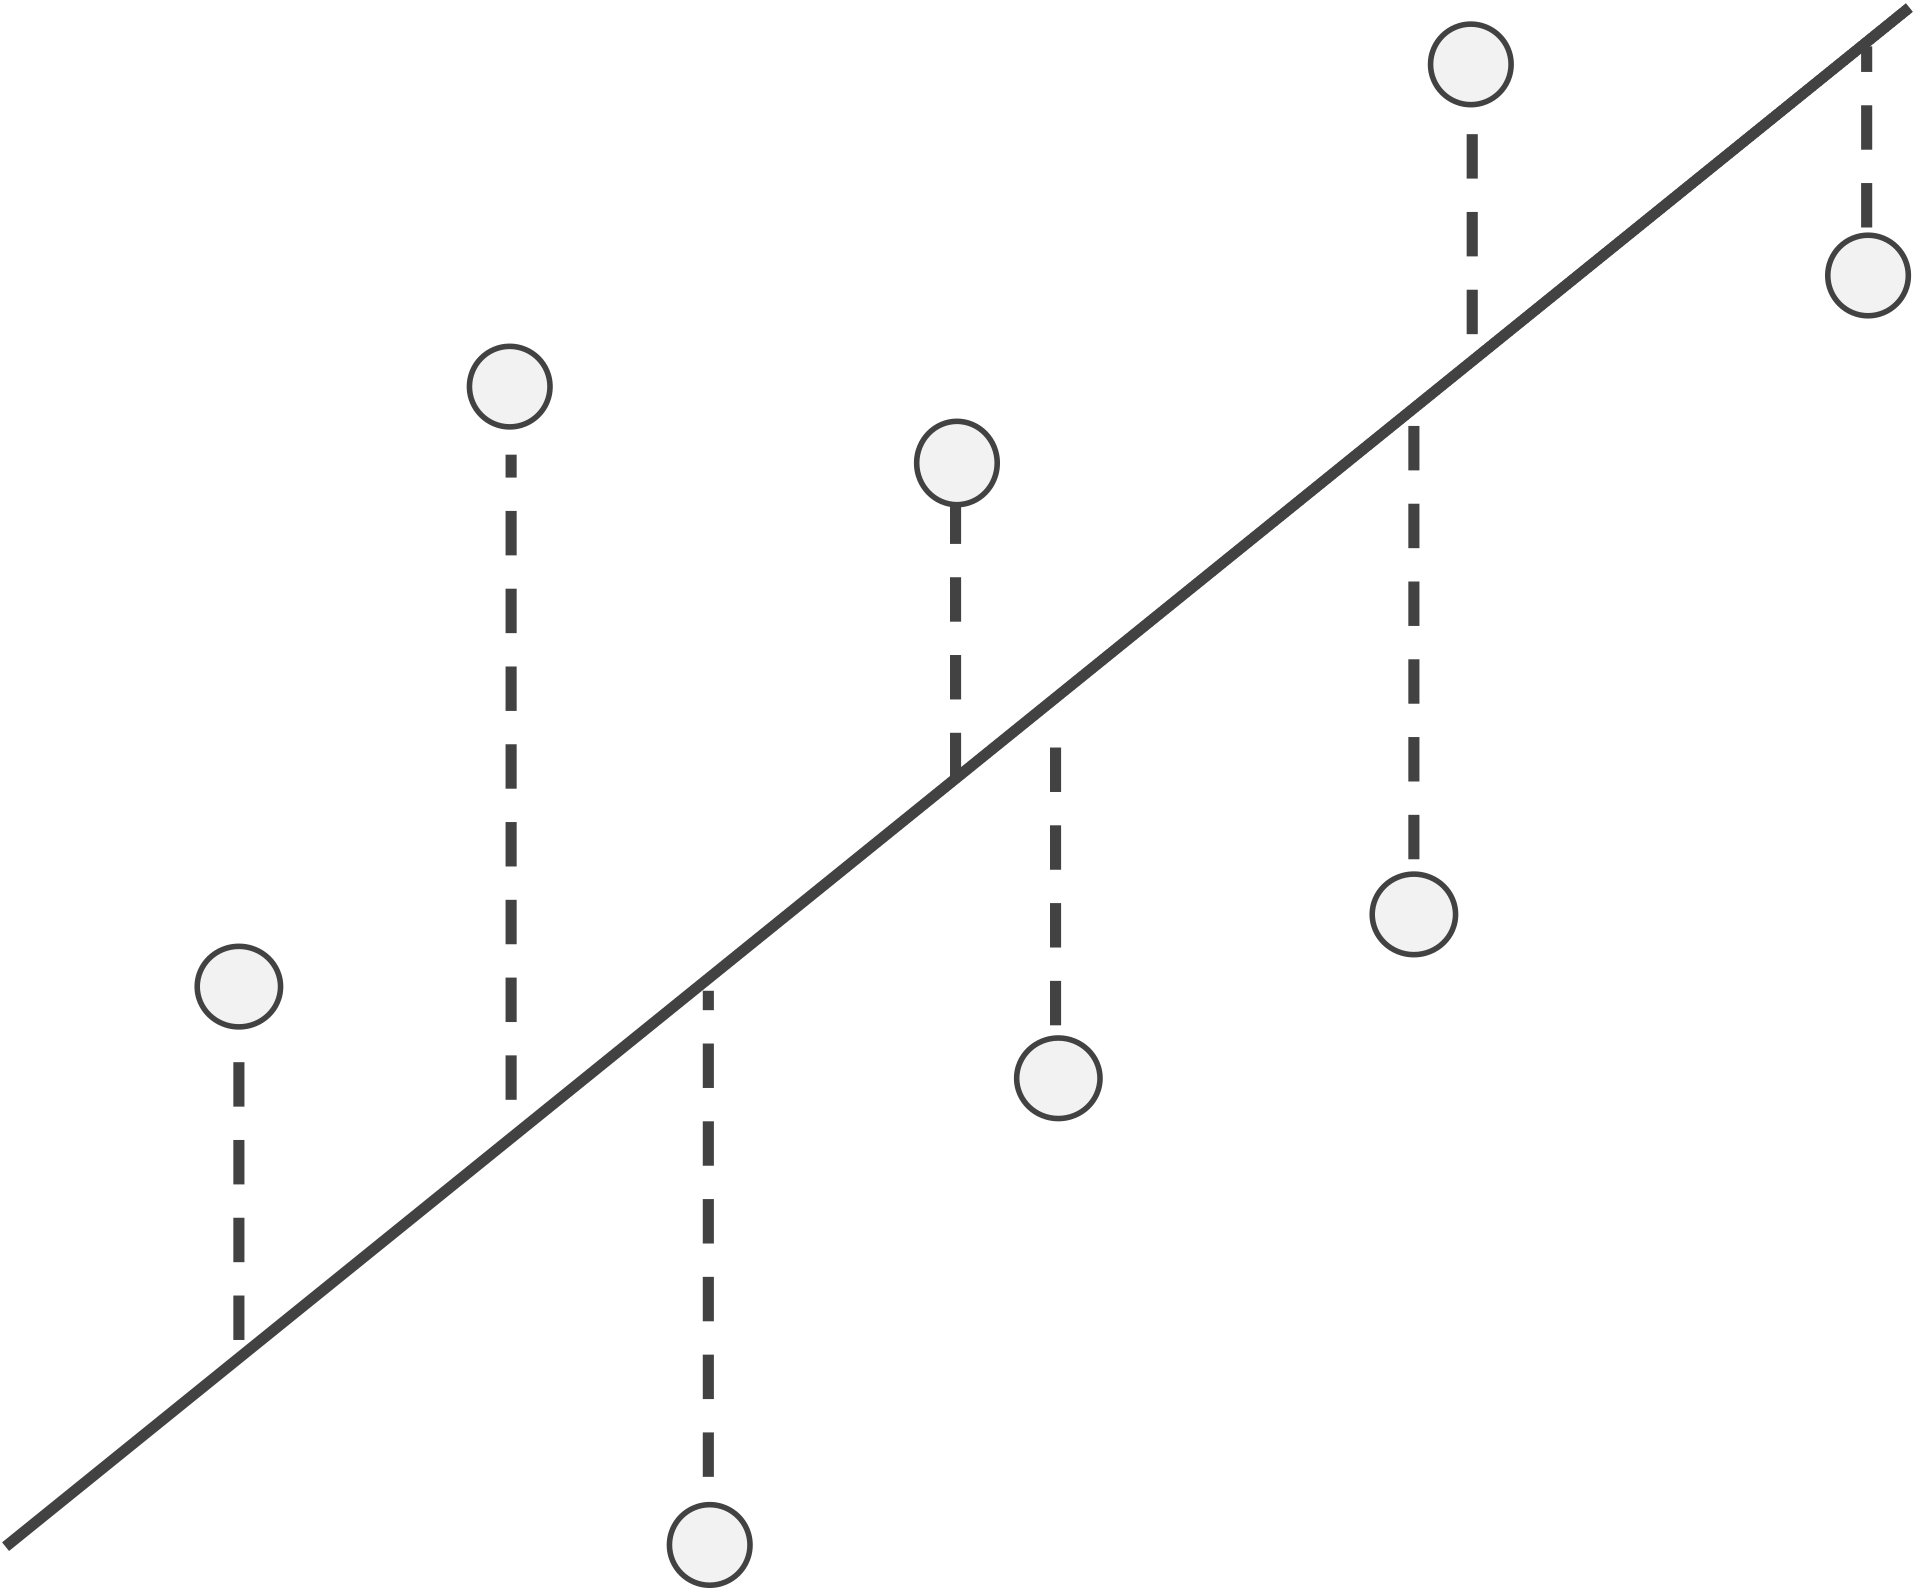
\includegraphics[width = 0.5\textwidth]{../images/residuals_y_coordinates.png}
\caption{An example line and data points with a visual depiction of the points' residuals. The absolute value of a residual is the length of its dashed line, and the sign of a residual corresponds to whether it lies above or below the line.}
\label{fig:residuals_y_coordinates}
\end{figure}

As the line changes, so will the points' residuals. The smaller the residuals become, the better the line fits the points. In linear regression, we are looking for the line that the line that minimizes the sum of squared residuals.

Linear regression is a common approach, but it is not the only way to fit a line to a collection of data. Choosing petal width as the dependent variable makes sense if we want to explain petal width as a function of petal length, but if we were to make petal length the dependent variable instead, then linear regression would minimize the squared differences between residuals in the x-direction, as illustrated in \autoref{fig:residuals_x_coordinates}.\\

\begin{figure}[h]
\centering
\mySfFamily
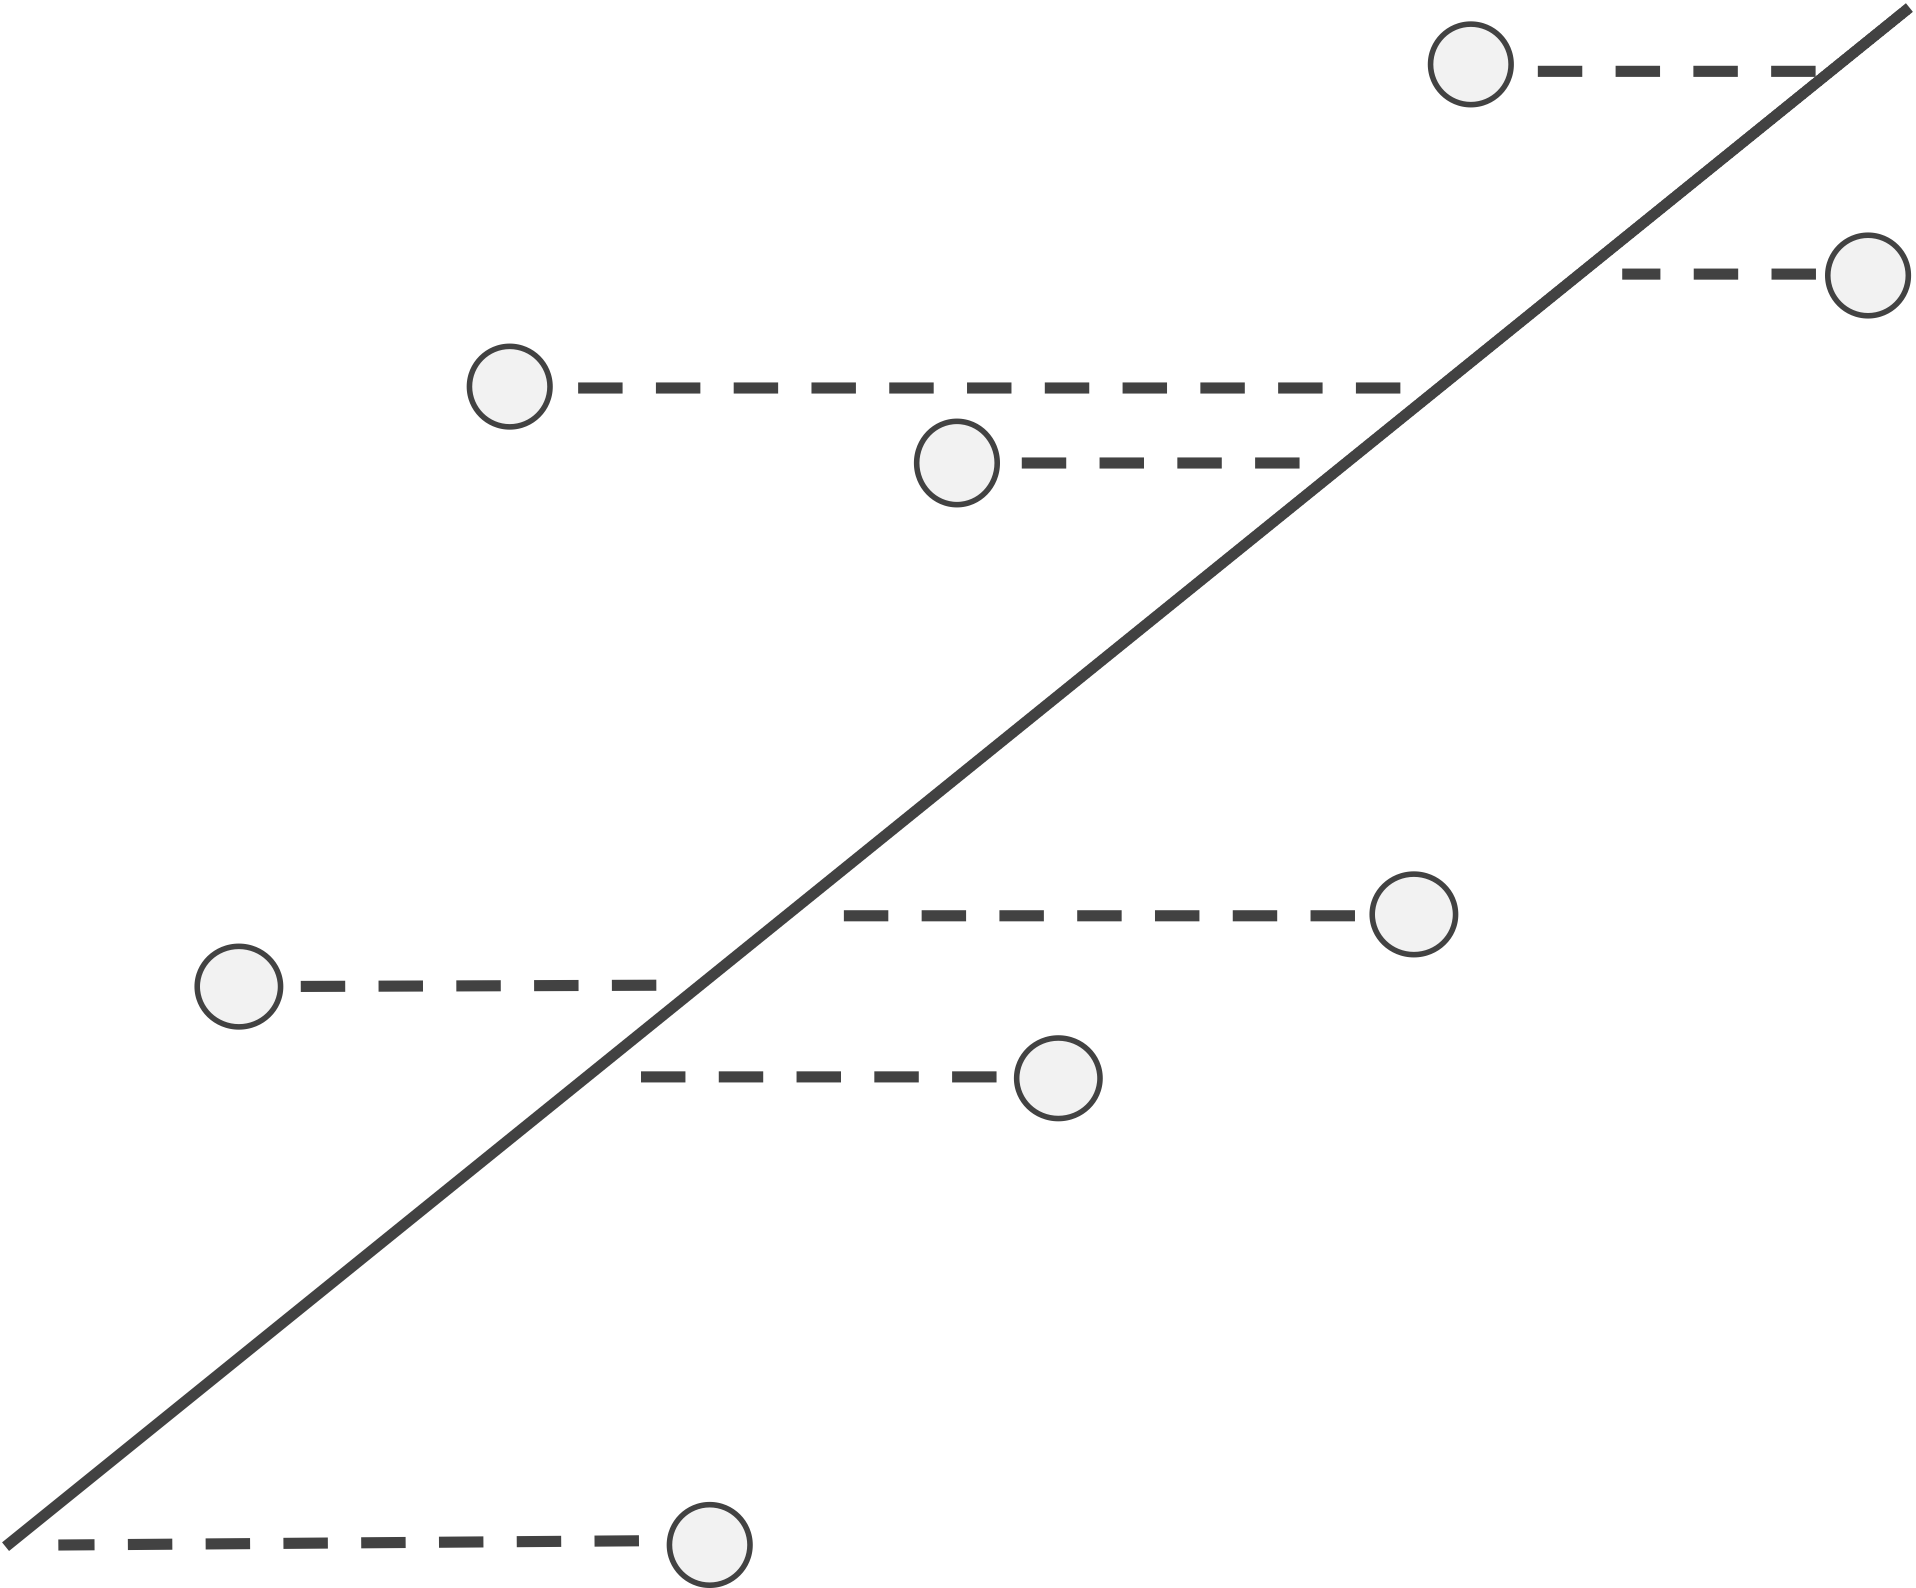
\includegraphics[width = 0.5\textwidth]{../images/residuals_x_coordinates.png}
\caption{If \textvar{x} is the dependent variable, then the residuals with respect to a line become the horizontal distances between points and the line, and linear regression finds the line that minimizes these horizontal residuals.}
\label{fig:residuals_x_coordinates}
\end{figure}

\begin{note}[%
The linear regression line will likely differ according to which variable we choose as the dependent variable, since the quantity that we are minimizing changes. However, if there is a linear pattern in our data, then the two regression lines will be similar.
]\end{note}

\fudgespace

\begin{qbox}[%
For the iris flower dataset, which of the two choices for dependent variable do you think is better?
]\end{qbox}

The preceding question is implying that no clear \textit{causality} underlies the correlation between petal width and petal length, which makes it difficult to prioritize one variable over the other as the dependent variable. For this reason, we will revisit how we are defining the line that best fits the data.

Instead of considering residuals based on distances to the line in only the x-direction or the y-direction, we can instead examine the distances from our data points to the line (\autoref{fig:residuals_projections}). The line minimizing the sum of the squares of these distances treats each of the two variables equally and is called the \textdefnogloss{first principal component} of the data.\\

\begin{figure}[h]
\centering
\mySfFamily
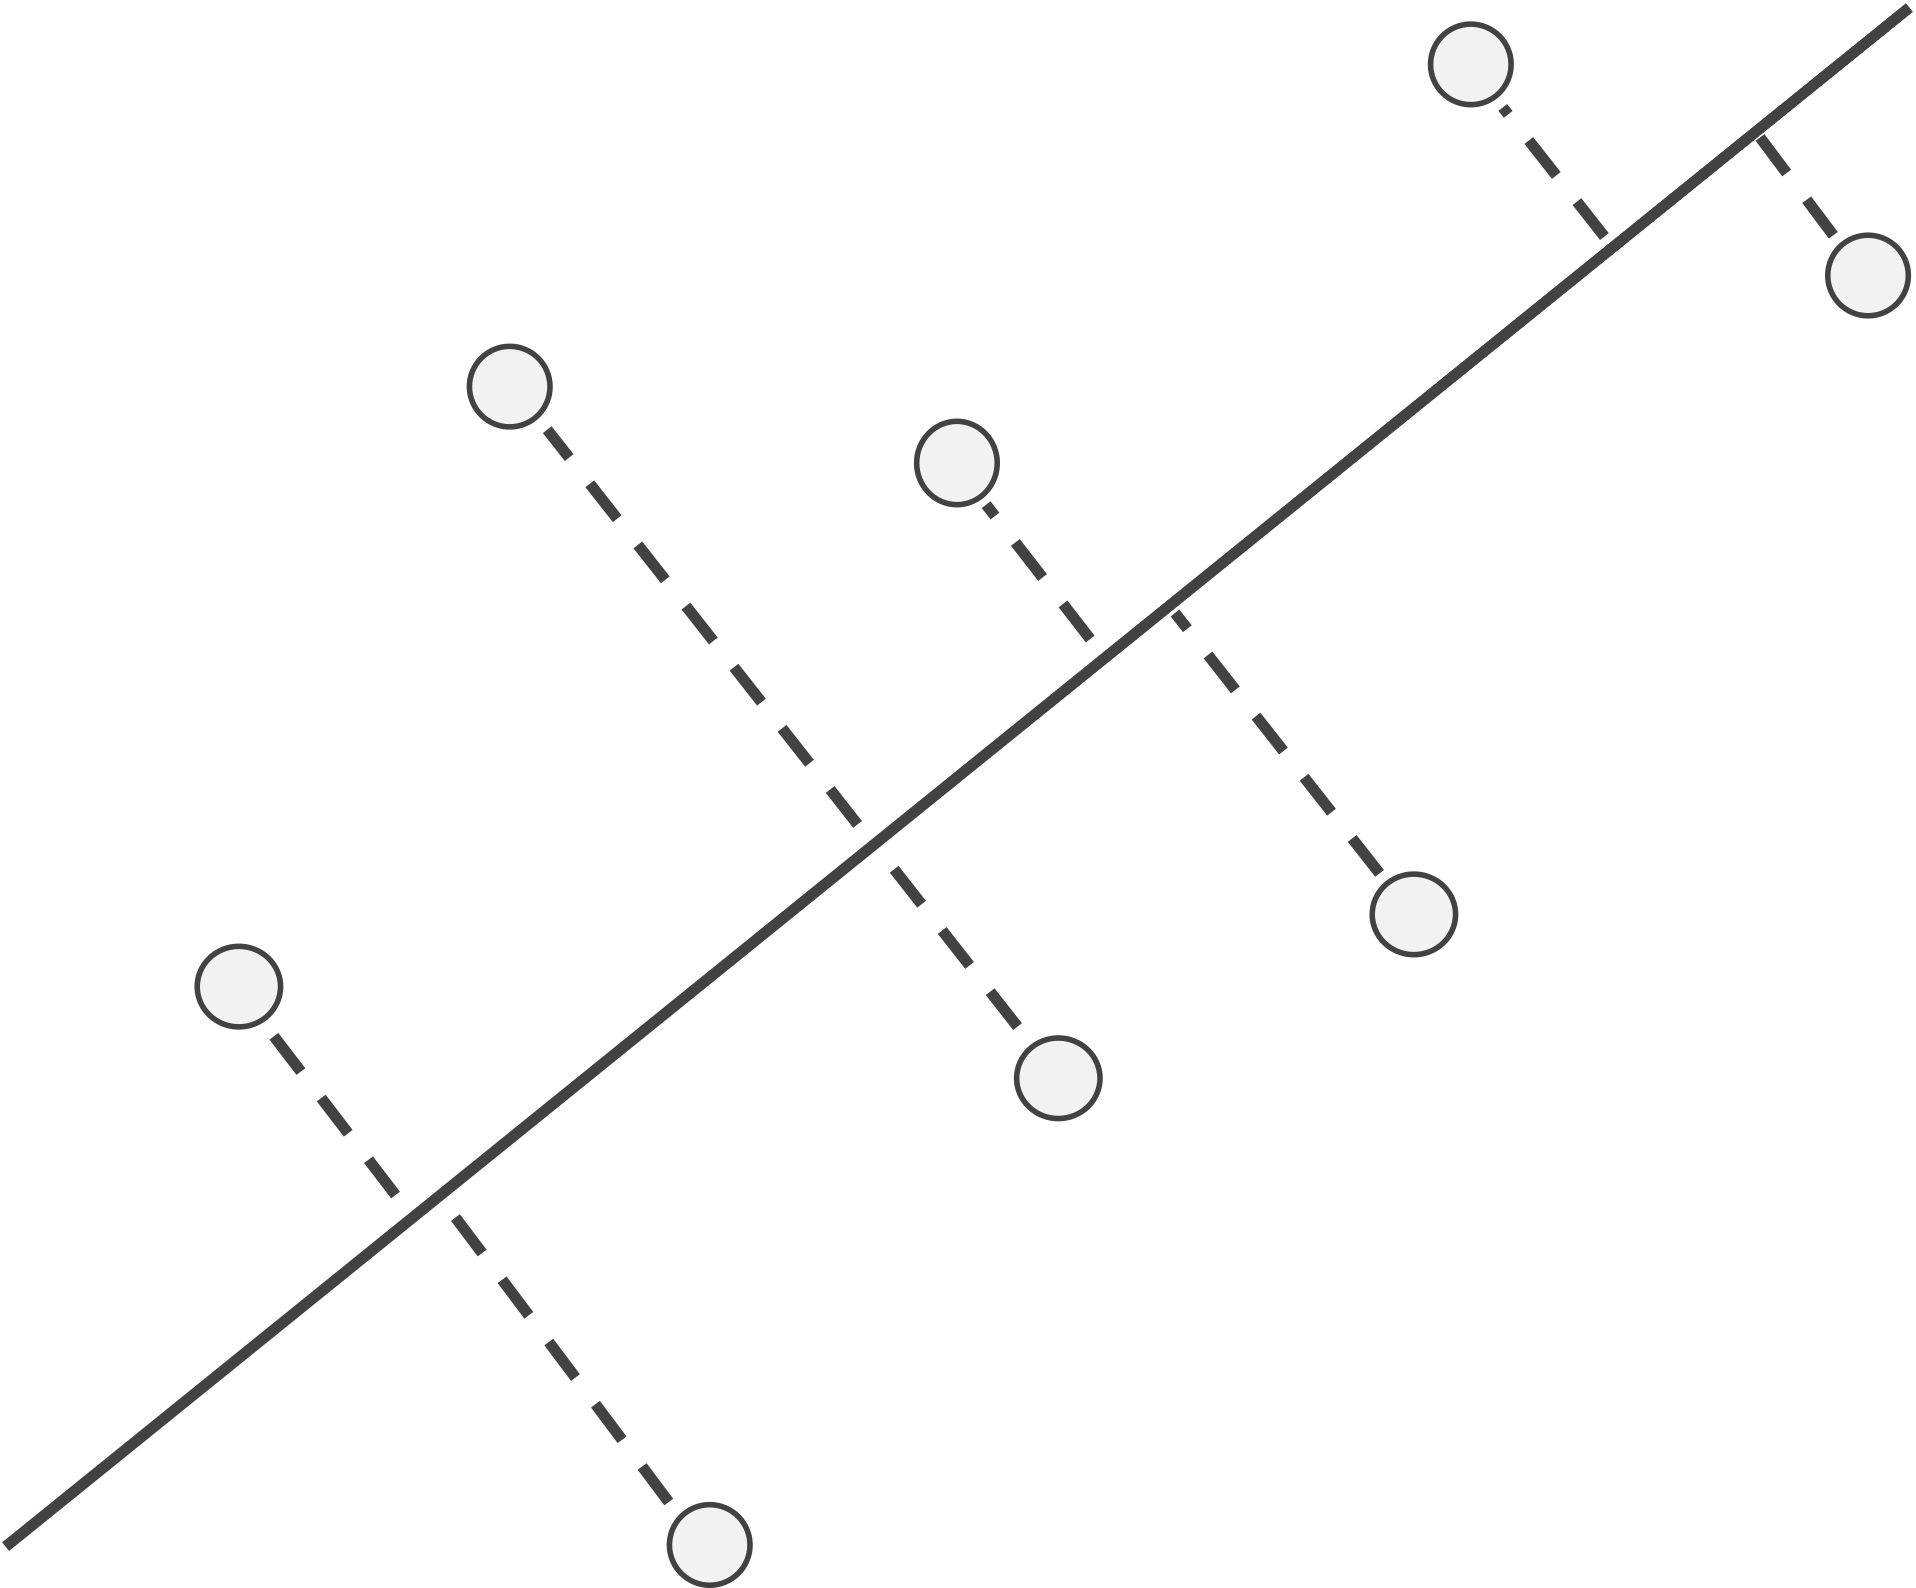
\includegraphics[width = 0.5\textwidth]{../images/residuals_projections.png}
\caption{A line along with a collection of points; dashed lines show the shortest segments connecting each point to the line.}
\label{fig:residuals_projections}
\end{figure}

The first principal component is often said to be the line that ``explains the most variance in the data''. If there is indeed a correspondence between lily petal width and length, then the distances from each point to the first principal component correspond to variation due to randomness. By minimizing the sum of squares of these distances, we limit the amount of variation in our data that we cannot explain.

%The following animated GIF shows a line rotating through a collection of data points, with the distance from each point to the line shown in red. As the line rotates, we can see the distances from the points to the line change.
%
%[![image-center](../assets/images/600px/pca_rotating_line_first_frame.png){: .align-center}](../assets/images/pca_rotating_line.gif)
%An animated GIF showing that the distances from points to their projections onto a line change as the line rotates. The line of best fit is the one in which the sum of the square of these distances is minimized.  Source: amoeba, StackExchange user.[^amoeba]
%{: style="font-size: medium;"}

Another benefit of finding the first principal component of a dataset is that it allows us to \textit{reduce} the dimensionality of our dataset from two dimensions to one. We call the point on a line that is nearest to a given point the \textdefnogloss{projection} of that point onto the line. As a result, the projections of a collection of data points onto their first principal component gives a one-dimensional representation of the data.

Say that we wanted to generalize the ideas above to three-dimensional space. The first principal component would offer a one-dimensional explanation of the variance in the data, but perhaps a line is insufficient to this end. Maybe the points all lie very near to a plane (a two-dimensional object), and projecting these points onto the nearest plane would effectively reduce the dataset to two dimensions.

Our three-dimensional minds will not permit us the intuition needed to visualize the extension of this idea into higher dimensions, but it is possible to generalize these concepts mathematically. Given a collection of \textvar{m} data points (vectors) in \textvar{n}-dimensional space, we are looking for a \textvar{d}-dimensional \textdef{hyperplane}{hyperplane}{an embedding of \textvar{d}-dimensional space inside \textvar{n}-dimensional space}, or an embedding of \textvar{d}-dimensional space inside \textvar{n}-dimensional space, such that the sum of squared distances from the points to the hyperplane is minimized. By taking the projections of points to their nearest point on this hyperplane, we reduce the dimension of the dataset from \textvar{n} to \textvar{d}. This approach, which is over 100 years old, is called \textdef{principal component analysis (PCA)}{principal component analysis (PCA)}{an approach used for finding the lower-dimensional hyperplane through a collection of data minimizing the distances of the points to the hyperplane}; a closely related concept called \textdefnogloss{singular value decomposition} was developed in the \nth{19} century.\\

\begin{note}[%
It can be shown that if $d_1$ is smaller than $d_2$, then the hyperplane provided by PCA of dimension $d_1$ is a subset of the hyperplane of dimension $d_2$. For example, the first principal component is always found within the plane ($d = 2$) provided by PCA.
]\end{note}

PCA may be old, but it is one of the fundamental tools of statistical analysis in an era defined by growing datasets. We will soon apply it to reduce the dimensions of our shape space; first, we make a brief aside to discuss a different biological problem in which the application of PCA has provided amazing insights.

\FloatBarrier
\phantomsection
\subsection{Genotyping: PCA is more powerful than you think}

Biologists have identified hundreds of thousands of \textdefnogloss{markers}, locations within human DNA that that are common sources of human variation. The most commonly type of marker is a single nucleotide (A, C, G, or T). In the process of \textdef{genotyping}{genotyping}{a process in which an individual's genetic markers are identified and compared to those sampled from others}, a service provided by companies as part of the booming ancestry industry, an individual's markers are determined from a DNA sample.

An individual's \textvar{n} markers can be converted to an \textvar{n}-dimensional vector $\mathbf{v} = (v_1, v_2, \ldots, v_n)$ such that $v_i$ is 1 if the individual possesses the variant for a marker and $v_i$ is 0 if the individual has the more common version of the marker.\\

\begin{note}[%
The mathematically astute reader will notice that this vector lies on one of the many corners of an \textvar{n}-dimensional hypercube.
]\end{note}

Because \textvar{n} is so large --- and in the early days of genotyping studies it far outnumbered the number of individual samples --- we need to be wary of the curse of dimensionality. When we apply PCA with $d = 2$ to produce a lower-dimensional projection of the data, we will see some amazing results that helped launch a multi-billion dollar industry.

\autoref{fig:genotyping_europe} shows a two-dimensional projection for individuals of known European ancestry. Even though we have condensed hundreds of thousands of dimensions to just two, and even though we are not capturing any information about the ancestry of the individuals other than their DNA, the projected data points reconstruct the map of Europe.\\

\begin{figure}[h]
\centering
\mySfFamily
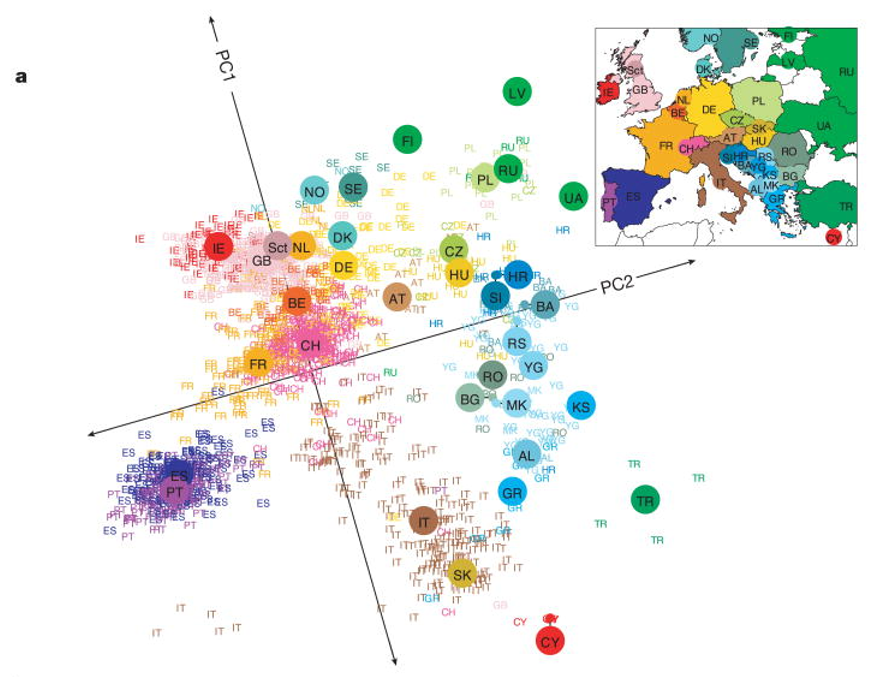
\includegraphics[width = 0.5\textwidth]{../images/genotyping_europe.png}
\caption{The projection of a collection of marker vectors sampled from individuals of known European ethnicity onto the plane produced by PCA with \textvar{d} = 2. Individuals cluster by country, and neighboring European countries remain nearby in the projected dataset. NEED courtesy}
\label{fig:genotyping_europe}
\end{figure}

If we zoom in on Switzerland, we can see that the countries around Switzerland tend to pull individuals toward them based on language spoken (\autoref{fig:genotyping_switzerland}).

\begin{figure}[h]
\centering
\mySfFamily
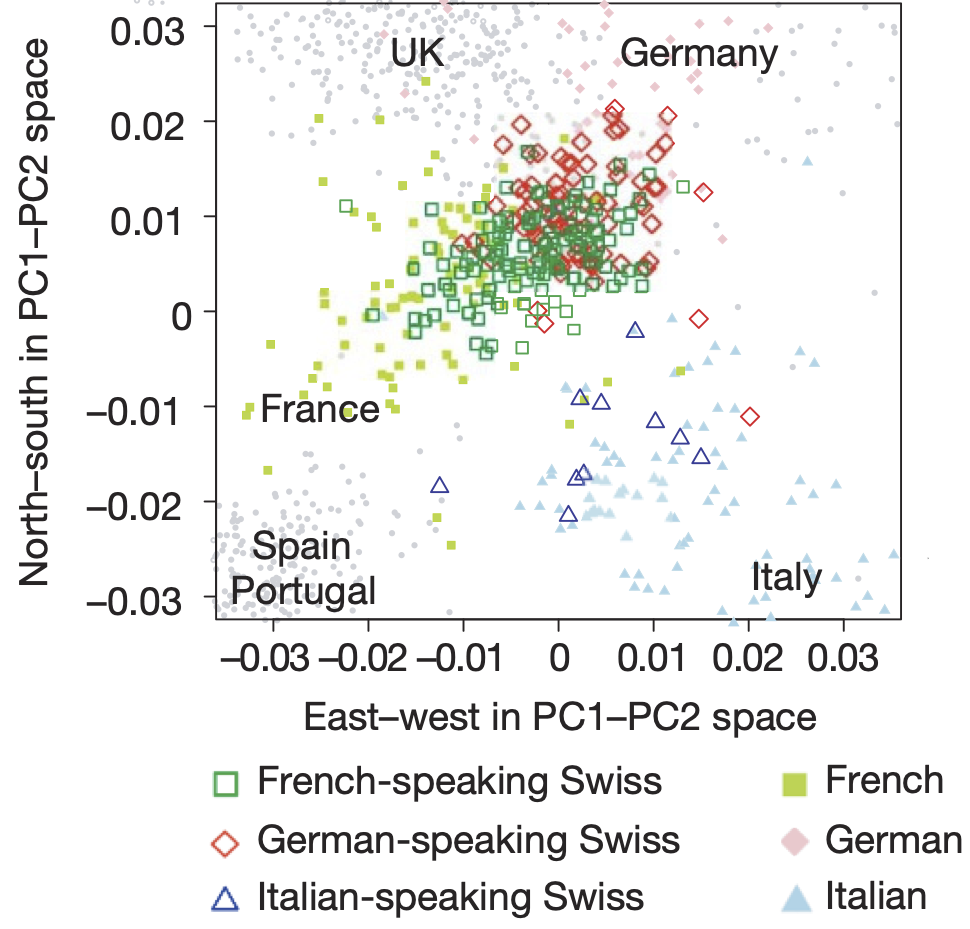
\includegraphics[width = 0.7\textwidth]{../images/genotyping_switzerland.png}
\caption{A PCA plot (\textvar{d} = 2) of individuals from Switzerland as well as neighboring countries shows that an individual's mother tongue correlates with the individual's genetic similarity to representatives from the neighboring country where that language is spoken. NEED courtesy}
\label{fig:genotyping_switzerland}
\end{figure}

And if we zoom farther out, then we can see continental patterns emerge, with India standing out as its own entity (\autoref{fig:genotyping_continents}). What is particularly remarkable about all these figures is that humans on the whole are genetically very similar, and yet PCA is able to find evidence of human migrations and separation lurking within our DNA.

\begin{figure}[h]
\centering
\mySfFamily
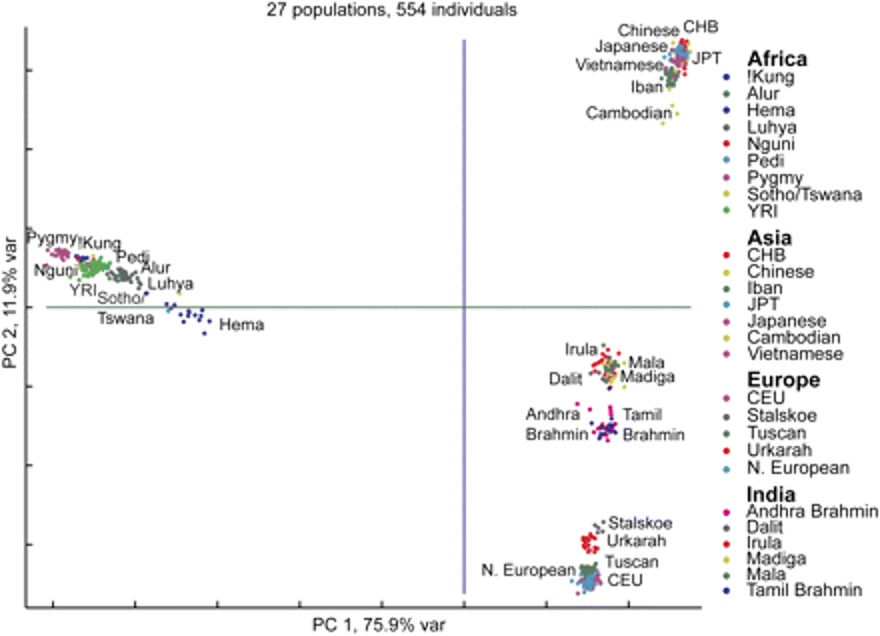
\includegraphics[width = 0.7\textwidth]{../images/genotyping_continents.png}
\caption{A PCA plot (\textvar{d} = 2) shows clustering of individuals from Europe, Asia, Africa, and India. NEED courtesy}
\label{fig:genotyping_continents}
\end{figure}

Now that we have established the power of PCA to help us see patterns in high-dimensional biological data, we are ready to use CellOrganizer to build a shape space for our WBC images and apply PCA to this shape space to produce a lower-dimensional representation of the space that we can visualize.\tutorial[https://biologicalmodeling.org/white_blood_cells/tutorial_shape_space]

\FloatBarrier
\phantomsection
\subsection{Visualizing the WBC shape space after PCA}

\autoref{fig:cellorg_pca_graph} shows the shape space of WBC images, reduced to three dimensions by PCA, in which each image is represented by a point that is color-coded according to its cell family.\\

\begin{figure}[h]
\centering
\mySfFamily
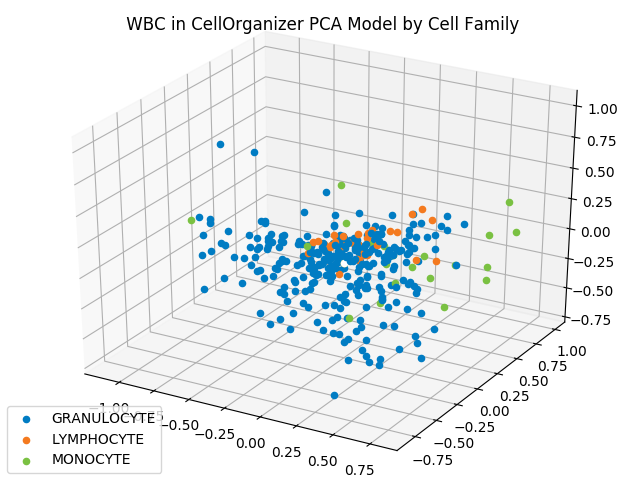
\includegraphics[width = 0.7\textwidth]{../images/cellorg_pca_graph.png}
\caption{The projection of each WBC shape vector onto a three-dimensional PCA hyperplane produces the above three-dimensional space. Granulocytes are shown in blue, lymphocytes are shown in orange, and monocytes are shown in green.}
\label{fig:cellorg_pca_graph}
\end{figure}

We can also subdivide granulocytes into basophils, eosinophils, and neutrophils. Updating our labels according to this subdivision produces the plot in \autoref{fig:cellorg_pca_graph_cell}.

\begin{figure}[h]
\centering
\mySfFamily
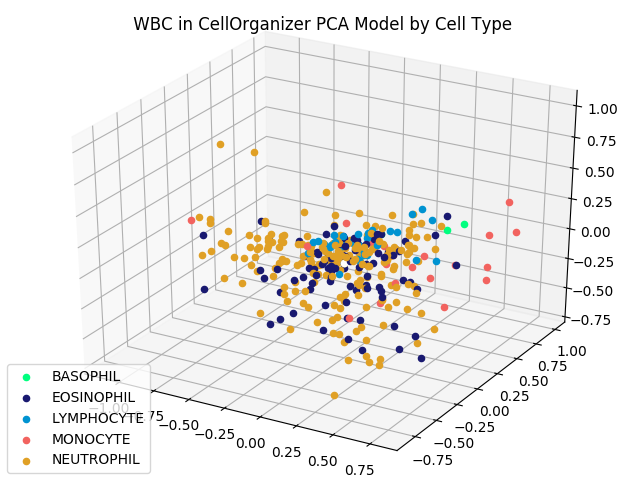
\includegraphics[width = 0.7\textwidth]{../images/cellorg_pca_graph_cell.png}
\caption{The reduced dimension shape space from the previous figure, with granulocytes subdivided into basophils, eosinophils, and neutrophils.}
\label{fig:cellorg_pca_graph_cell}
\end{figure}

Although images from the same family do not cluster as tightly as the iris flower dataset --- which could be criticized as an unrealistic representation of the noise inherent in most real datasets --- images from the same type do appear to be nearby. This fact should give us hope that proximity in a dimension-reduced space may help us correctly classify images of unknown type.

\FloatBarrier
\phantomsection

\section{Classifying White Blood Cell Images}
\label{sec:training}

\phantomsection
\subsection{Cross validation}

We would like to apply k-NN to a dimension-reduced shape space WBC images to see how often it assigns an image to the correct class. The tricky part is that we already know the correct class for every image in our dataset. To get around this issue, we could exclude some \textit{subset} of the data, called the \textdefnogloss{validation set}. After pretending that we don't know the correct classes for elements of the validation set, we will see how often our classification algorithm correctly identifies the class of each object in this set.\\

\begin{qbox}[%
What issues do you see with using a validation set?
]\end{qbox}

Unfortunately, it is unclear which subset of the data we should use as a validation set. Random variation could mean that the reported accuracy will change depending on which subset we choose. And what makes the elements of the validation set so special as to be chosen? Ideally, we would use a more democratic approach that is not subject to random variation and that uses \textit{all} of the data for validation.

In \textdef{cross validation}{cross validation}{an approach used in classification (or other machine learning approaches) in which we divide the data into approximately equally sized groups called folds; over multiple rounds, one fold is used as a validation set, pretending that we do not know the correct class of these data points, and we measure the correctness of the approach at identifying the class of each point}, we divide our data into a collection of \textvar{f} (approximately) equally sized groups called \textdefnogloss{folds}. We use one of these folds as a validation set, keeping track of how many objects are correctly classified, and then we start over with a different fold as our validation set. Cross validation is democratic, since every element in our dataset will get used as a member of a validation set exactly once.

The case in which \textvar{f} is equal to the number of points in our dataset is called \textdefnogloss{leave one out cross validation}. For every point in the dataset, we pretend that we do not know its label, use the classification algorithm to assign it a class, and then compare this prediction against the known class.

\FloatBarrier
\phantomsection
\subsection{A first attempt at quantifying the success of a classifier}

Before we can apply cross validation to WBC images, we should know how to quantify the performance of the classifier. This task may seem easy, but we will see that pitfalls are lurking.

\autoref{fig:iris_confusion_matrix} shows the result of applying k-NN to the iris flower dataset, using \textvar{k} equal to 1 and cross-validation with \textvar{f} equal to 10 (meaning that since there are 150 flowers, each fold contains 15 flowers). This table is called a \textdef{confusion matrix}{confusion matrix}{a table used to measure the results of a classification algorithm, identifying how many items from each known class were assigned to each class by the algorithm}, because it helps us visualize whether we are ``confusing'' the assignment of a flower to the wrong class.\\

\begin{figure}[h]
\centering
\tabcolsep = 1 em
\mySfFamily
\begin{tabular}{c c c}
\textbf{\textit{Iris setosa}} & \textbf{\textit{Iris versicolor}} & \textbf{\textit{Iris virginica}} \\
50 & 0 & 0 \\
0 & 47 & 3 \\
0 & 4 & 46
\end{tabular}
\caption{The confusion matrix that is the result of applying k-NN to the iris flower dataset, using $\textvar{k} = \text{1}$ and cross-validation with $\textvar{f} = \text{10}$.}
\label{fig:iris_confusion_matrix}
\end{figure}

In the confusion matrix, rows correspond to true classes, and columns correspond to predicted classes. For example, consider the second row in \autoref{fig:iris_confusion_matrix}, which corresponds to the flowers that we know are \textit{Iris versicolor}. Our classifier predicted that none of these flowers were \textit{Iris setosa}, that 47 of these flowers were \textit{Iris versicolor}, and that three of the flowers were \textit{Iris virginica}. Therefore, it correctly predicted the class of 47 of the 50 total \textit{Iris versicolor} flowers.\\

\begin{note}[%
We did not apply dimension reduction to the iris flower dataset because it has only four dimensions.
]\end{note}

We define the \textdef{accuracy}{accuracy}{the fraction of data points that a classification algorithm correctly classifies out of the total number of data points} of a classifier as the fraction of objects that it correctly identifies out of the total. For the above iris flower example, the confusion matrix indicates that k-NN has an accuracy of $(50 + 47 + 46)/150 = 95.3\%$.

It may seem that accuracy is the only metric that we need. But if you were in a smarmy mood, then you might design a classifier that produces the confusion matrix in \autoref{fig:wbc_clown_matrix} for our WBC dataset.\\

\begin{figure}[h]
\centering
\tabcolsep = 1 em
\mySfFamily
\begin{tabular}{c c c}
\textbf{Granulocyte} & \textbf{Monocyte} & \textbf{Lymphocyte} \\
291 & 0 & 0 \\
21 & 0 & 0 \\
33 & 0 & 0
\end{tabular}
\caption{The confusion matrix for our WBC image dataset corresponding to assigning every image as a granulocyte.}
\label{fig:wbc_clown_matrix}
\end{figure}

\begin{qbox}[%
What is the accuracy of this classifier?
]\end{qbox}

The clown classifier blindly assigned every image in the dataset to be a granulocyte. And yet its accuracy is $291/345 = 84.3\%$! To make matters worse, \autoref{fig:wbc_better_confusion_matrix} shows a confusion matrix for a hypothetical classifier on the same dataset that is clearly better. And yet its accuracy would be only $(232 + 17 + 26)/345 = 79.7\%$.\\

\begin{figure}[h]
\centering
\tabcolsep = 1 em
\mySfFamily
\begin{tabular}{c c c}
\textbf{Granulocyte} & \textbf{Monocyte} & \textbf{Lymphocyte} \\
232 & 25 & 34 \\
2 & 17 & 2 \\
6 & 1 & 26
\end{tabular}
\caption{A hypothetical confusion matrix for our WBC image dataset.}
\label{fig:wbc_better_confusion_matrix}
\end{figure}

The failure of this classifier to attain the same accuracy as the one assigning the majority class to each element owes to the WBC dataset having \textit{imbalanced} classes, a common issue in data science. Imbalanced classes mean that only reporting a classifier's accuracy may be misleading.

For another example, say that we design a sham COVID test that always comes back negative. If 1\% of the population at a given point in time is COVID-positive, then we could report that our test is 99\% accurate. But we would fail to get this test approved for widespread use because it performs horribly on COVID-positive individuals.\\

\begin{qbox}[%
What other metrics could we design for measuring the success of a classifier?
]\end{qbox}

\FloatBarrier
\phantomsection
\subsection{Recall, specificity, and precision}

To motivate our discussion of other classifier metrics, we will continue discussing medical tests, which can be thought of as classifiers with two classes (positive or negative).

First, we define some terms. A \textdef{true positive}{true positive}{a positive test in an individual that is positive for the condition} is a positive test in a patient that has the disease; a \textdef{false positive}{false positive}{a positive test in an individual that is negative for the condition} is a positive test in a patient that does not have the disease; a \textdef{true negative}{true negative}{a negative test in an individual that is negative for the condition} is a negative test in a patient that does not have the disease; and a \textdef{false negative}{false negative}{a negative test in an individual that is positive for the condition} is a negative test in a patient that does have the disease. \autoref{fig:medical_test_confusion_matrix} shows the locations of these four terms in a two-class confusion matrix.\\

\begin{figure}[h]
\centering
\mySfFamily
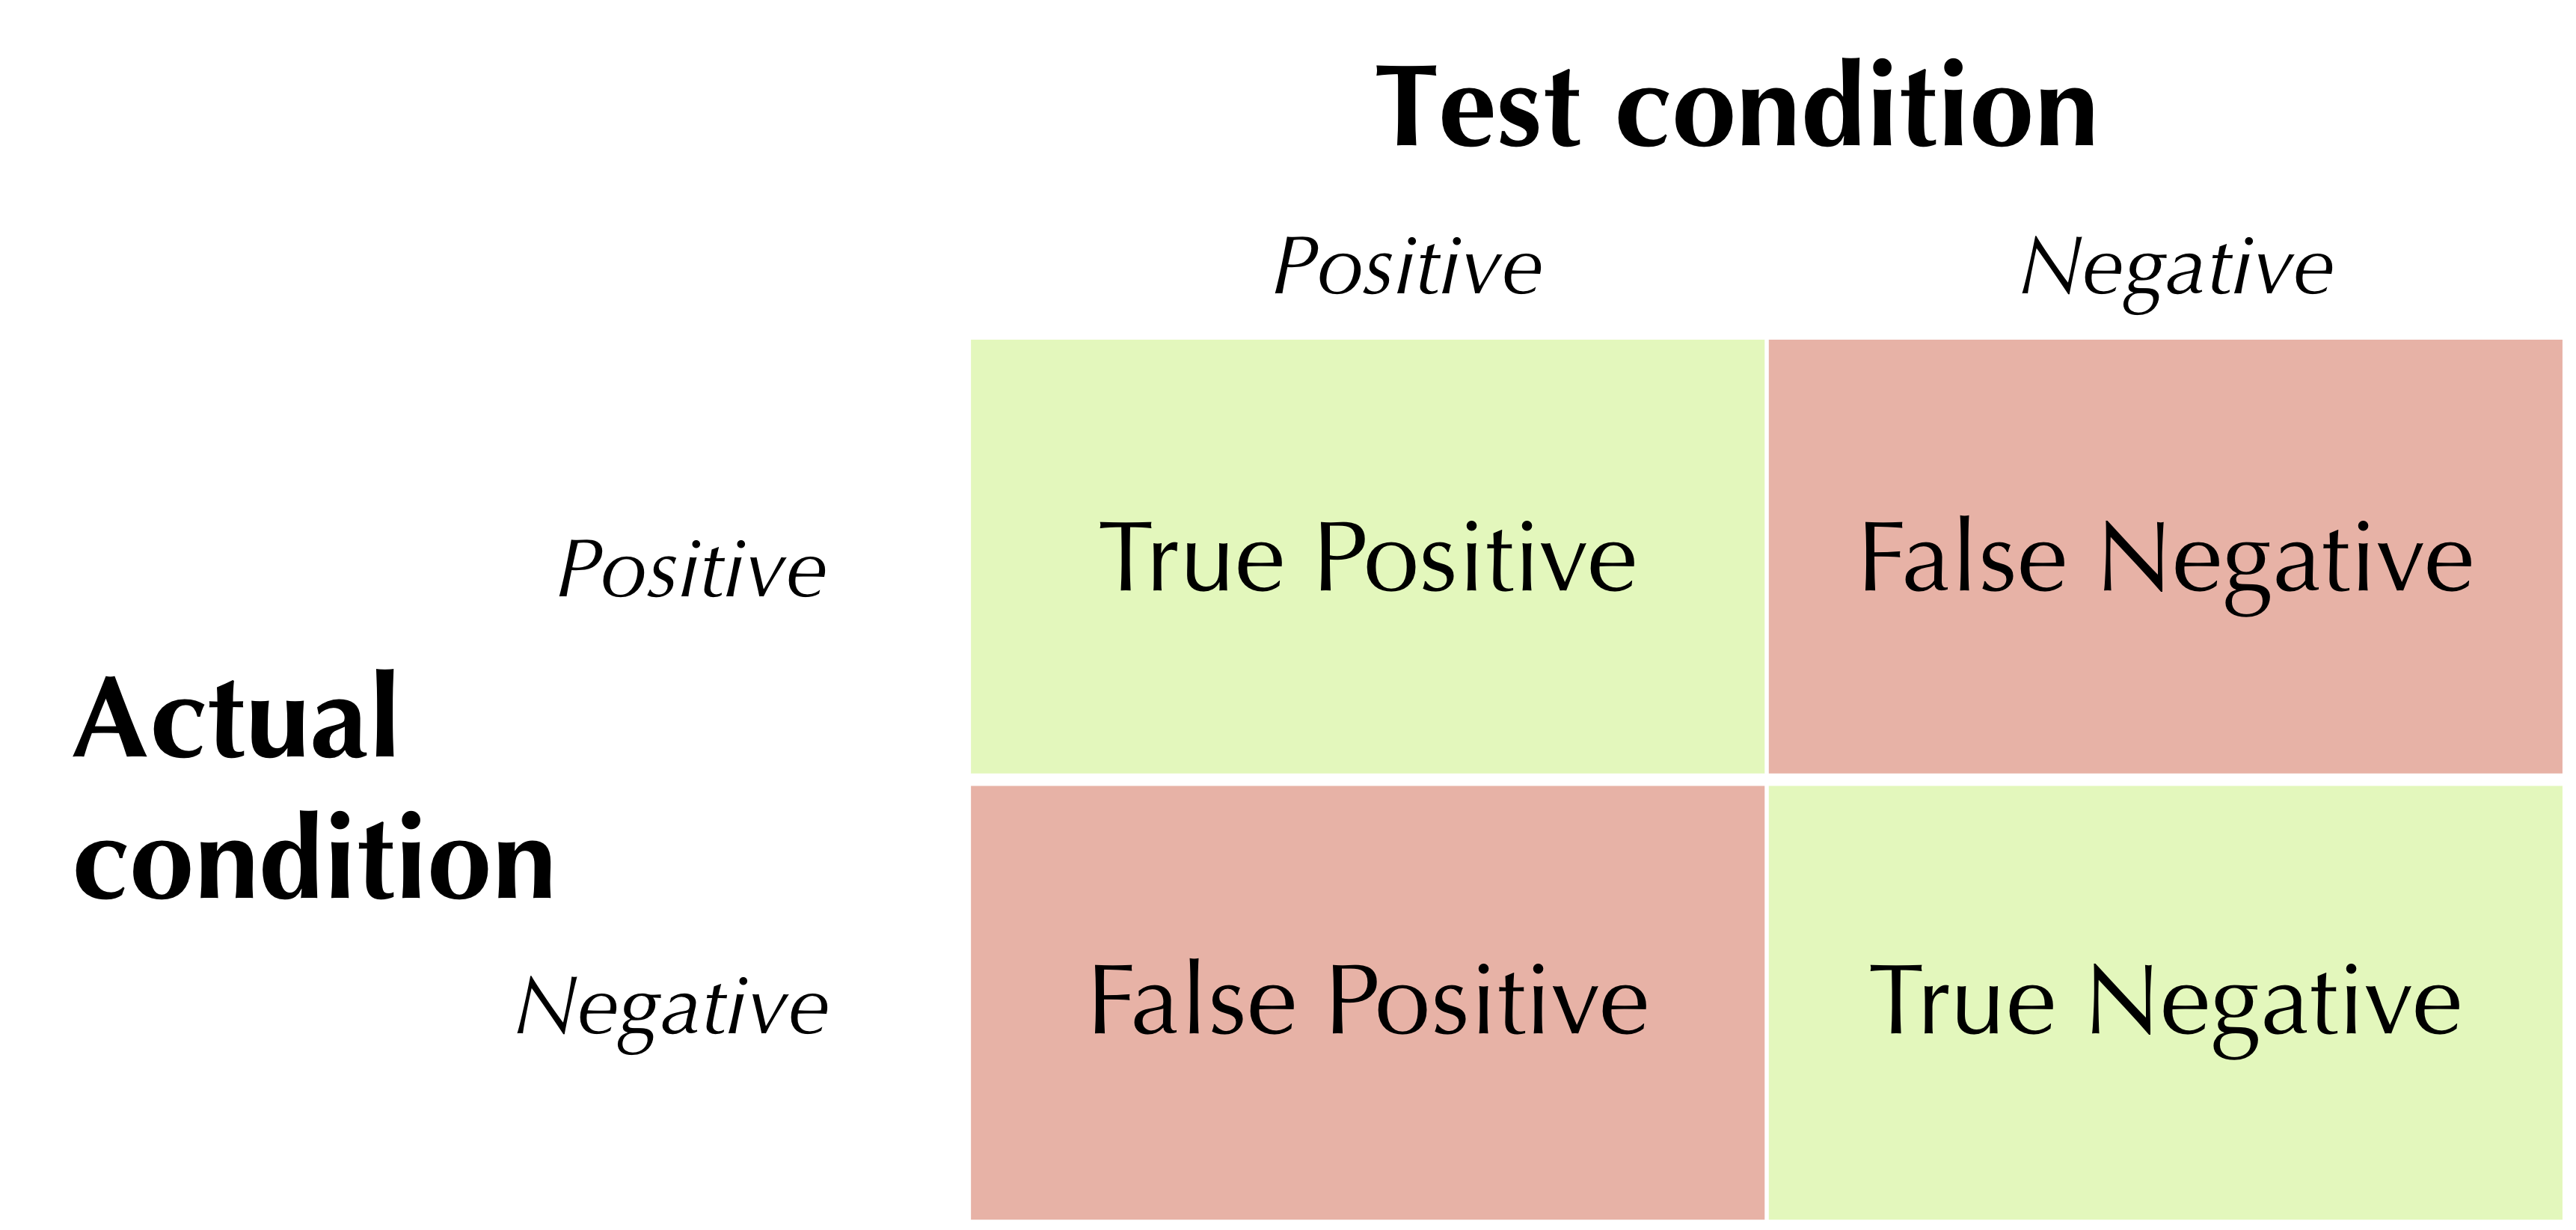
\includegraphics[width = 0.7\textwidth]{../images/medical_test_confusion_matrix.png}
\caption{The locations of true positives, true positives, true negatives, and false negatives in the confusion matrix associated with a medical test. Correct predictions are shown in green, and incorrect predictions are shown in red.}
\label{fig:medical_test_confusion_matrix}
\end{figure}

In what follows, we will use the hypothetical confusion matrix for a COVID test shown in \autoref{fig:medical_test_confusion_matrix_hypothetical}. We used a hypothetical confusion matrix because results for COVID tests, even the same type of test, can vary widely.\\

\begin{figure}[h]
\centering
\mySfFamily
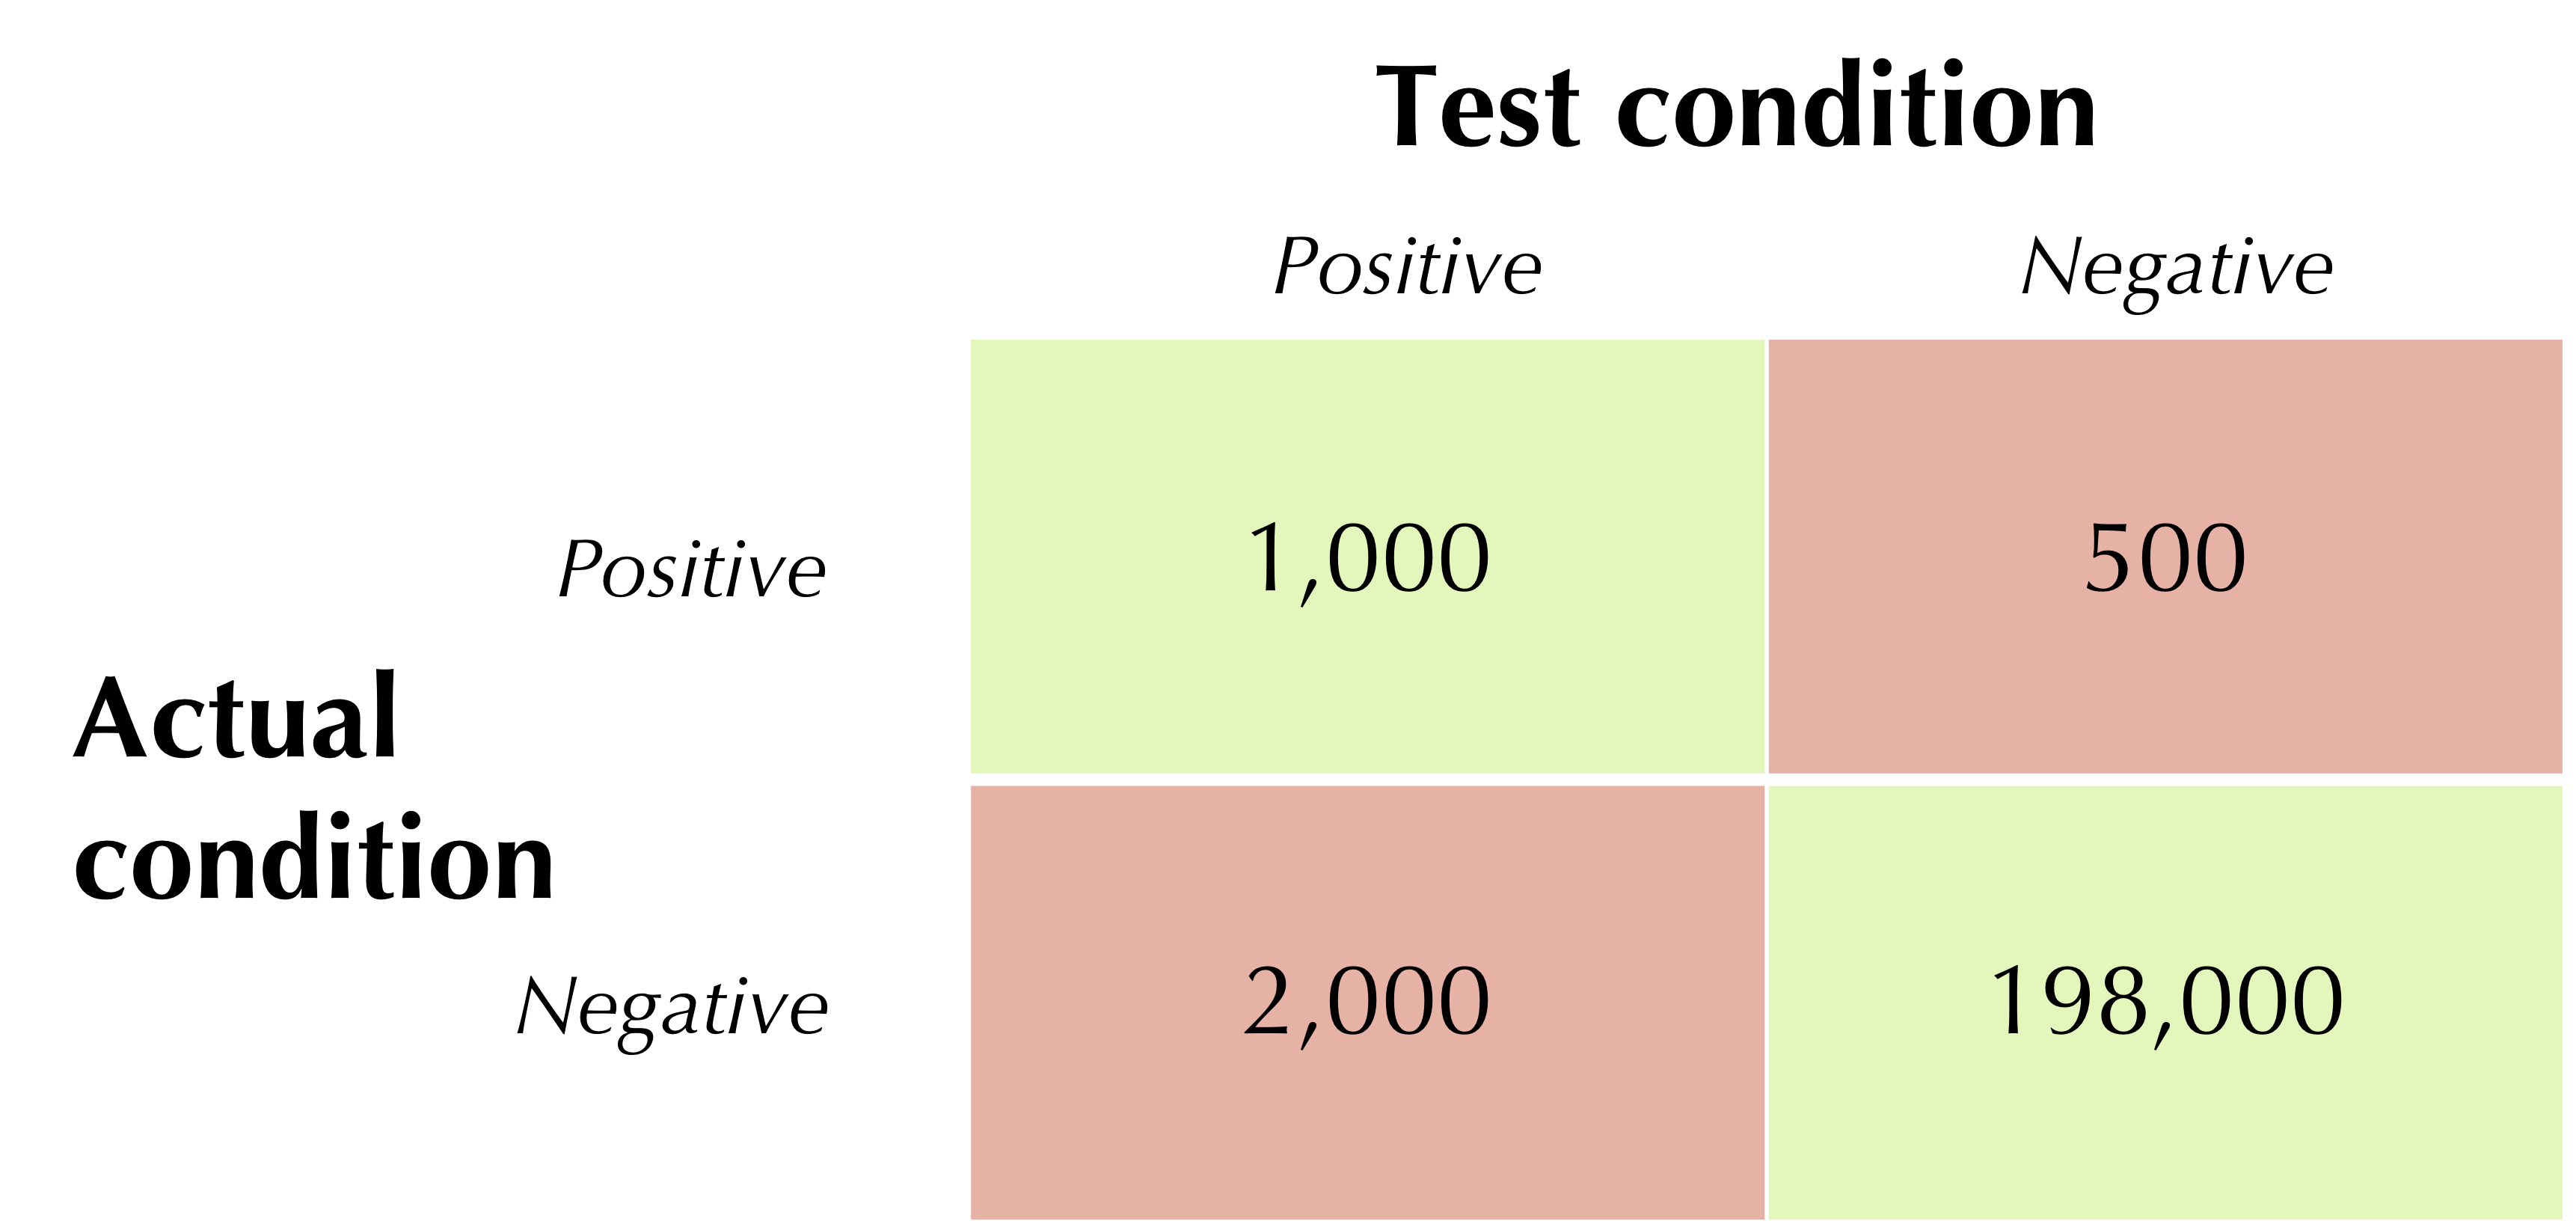
\includegraphics[width = 0.7\textwidth]{../images/medical_test_confusion_matrix_hypothetical.png}
\caption{A hypothetical COVID test confusion matrix.}
\label{fig:medical_test_confusion_matrix_hypothetical}
\end{figure}

\begin{qbox}[%
What is the accuracy of this test? How does it compare to the accuracy of a test that returns negative for everyone in the population?
]\end{qbox}

Once again, this test has lower accuracy than one that returns negative for all individuals, but we will now show metrics for which it is superior.

The \textdef{recall}{recall (sensitivity)}{the percentage of positive cases that a two-class classifier such as a medical test correctly identifies, or the ratio of true positives over the sum of the true positives and false negatives} (a.k.a.~\textdefnogloss{sensitivity}) of a two-class classifier is the percentage of positive cases that the test correctly identifies, or the ratio of true positives over the sum of the true positives and false negatives (found by summing the top row of the confusion matrix). For our hypothetical COVID confusion matrix in \autoref{fig:medical_test_confusion_matrix_hypothetical}, the recall is $1,000/(1,000 + 500) = 66.7\%$. Recall ranges from 0 to 1, with larger values indicating that the test is ``sensitive'', meaning that it can identify true positives out of patients who actually are positive.

The \textdef{specificity}{specificity}{the ratio of true negatives to the sum of true negatives and false positives for a two-class classifier such as a medical test} of a test is an analogous metric for patients whose actual status is negative. It measures the ratio of true negatives to the sum of true negatives and false positives (found by summing the second row of the confusion matrix). For the test with confusion matrix in \autoref{fig:medical_test_confusion_matrix_hypothetical}, the test specificity is $198,000/(198,000 + 2,000) = 99\%$.

Finally, the \textdef{precision}{precision}{the percentage of positive tests that are correct for a two-class classifier such as a medical test, formed by taking the ratio of true positives to the sum of true positives and false positives} of a test is the percentage of positive tests that are correct, formed by taking the ratio of true positives to the sum of true positives and false positives (found by summing the first column of the confusion matrix). For example, the  test whose confusion matrix is shown in \autoref{fig:medical_test_confusion_matrix_hypothetical} is $1,000/(1,000 + 2,000) = 33.3\%$.\\

\begin{qbox}[%
How could we trick a test to have recall close to 1? What about specificity or precision?
]\end{qbox}

Just like accuracy, all three of the metrics we have just introduced are imperfect and can be fooled by frivolous tests that always return positive or negative. However, it is not possible for such a test to score well on all of these metrics at the same time. Therefore, in practice we will examine all of these metrics, as well as accuracy, when assessing the quality of a classifier.\\

\begin{qbox}[%
Compute the recall, specificity, and precision of a hypothetical COVID test that always returns negative.
]\end{qbox}

You may find all these terms confusing and difficult to keep straight. You are not alone! An entire generation of scientists make copious trips to the \href{https://en.wikipedia.org/wiki/Precision_and_recall#Definition_(classification_context)}{Wikipedia page} describing these metrics as well as others used for analyzing classifiers. After all, it's called a confusion matrix for a reason\ldots

\FloatBarrier
\phantomsection
\subsection{Extending classification metrics to multiple classes}

To return to our example of classifying images of WBC nuclei, we need to extend the ideas discussed in the preceding section to handle more than two classes. To do so, we consider each class individually and treat this class as the ``positive'' case.

We use the iris flower dataset to show how this works. Say that we wish to compute the recall, specificity, and precision for \textit{Iris virginica} using the k-NN confusion matrix in \autoref{fig:iris_confusion_matrix}. We can simplify this confusion matrix into a two-class confusion matrix that combines the two classes corresponding to the other two species. \autoref{fig:iris_confusion_matrix_compressed}
 shows this smaller confusion matrix, with \textit{Iris virginica} moved to the first row and column.\\

 \begin{figure}[h]
\centering
\tabcolsep = 1 em
\mySfFamily
\begin{tabular}{c c}
\textbf{\textit{Iris virginica}} & \textbf{\textit{Iris setosa} and \textit{Iris versicolor}} \\
46 & 4 \\
3 & 47 \\
\end{tabular}
\caption{A compressed version of the confusion matrix in \autoref{fig:iris_confusion_matrix} in which we combine \textit{Iris setosa} and \textit{Iris versicolor} into a single class.}
\label{fig:iris_confusion_matrix_compressed}
\end{figure}

This simplification allows us to compute the recall, specificity, and precision for ths classifier with respect to \textit{Iris virginica}.

\begin{itemize}
\item recall: $46/(46+4) = 92\%$
\item specificity: $47/(3+47) = 94\%$
\item precision: $46/(46+3) = 93.9\%$
\end{itemize}

\fudgespace

\begin{qbox}[%
Compute the recall, specificity, and precision for each of the other two iris species using the confusion matrix in \autoref{fig:iris_confusion_matrix}.
]\end{qbox}

Now that we understand more about how to quantify the performance of a classifier, we are ready to apply k-NN to our WBC shape space --- post-PCA of course! --- and assess its performance.\tutorial[https://biologicalmodeling.org/white_blood_cells/tutorial_image_classification]

\FloatBarrier
\phantomsection
\subsection{Applying a classifier to the WBC shape space}

If we run k-NN on our shape space, using \textvar{d} (the number of dimensions in the PCA hyperplane) equal to 10, \textvar{k} (the number of nearest neighbors to consider when assigning a class) equal to 1, and \textvar{f} (the number of folds) equal to 10, then we obtain the confusion matrix shown in \autoref{fig:wbc_better_confusion_matrix}. For this dataset, k-NN has an accuracy of 84.3\% and a weighted average of precision and recall over all three classes of 85.7\% and 84.3\%, respectively.\\

\begin{figure}[h]
\centering
\tabcolsep = 1 em
\mySfFamily
\begin{tabular}{c c c}
\textbf{Granulocyte} & \textbf{Monocyte} & \textbf{Lymphocyte} \\
259 & 9 & 23 \\
14 & 6 & 1 \\
5 & 2 & 26
\end{tabular}
\caption{The confusion matrix for our WBC image dataset using k-NN with $\textvar{d} = \text{10}$, $\textvar{k} = \text{1}$, and $\textvar{f} = \text{10}$.}
\label{fig:wbc_better_confusion_matrix}
\end{figure}

These three values of \textvar{d}, \textvar{k}, \textvar{f} appear to be close to optimal, in that changing them does not improve our classification metrics. We should ask why this is the case.

We start with \textvar{d}. If we set \textvar{d} too large, then once again the curse of dimension strikes. Using \textvar{d} equal to 344 (with \textvar{k} equal to 1 and \textvar{f} equal to 10) produces the baffling confusion matrix in \autoref{fig:wbc_baffling_confusion_matrix}, in which every element in the space is somehow closest to a lymphocyte.

\begin{figure}[h]
\centering
\tabcolsep = 1 em
\mySfFamily
\begin{tabular}{c c c}
\textbf{Granulocyte} & \textbf{Monocyte} & \textbf{Lymphocyte} \\
0 & 0 & 291 \\
0 & 0 & 21 \\
0 & 0 & 33
\end{tabular}
\caption{The confusion matrix for our WBC image dataset using k-NN with $\textvar{d} = \text{344}$, $\textvar{k} = \text{1}$, and $\textvar{f} = \text{10}$.}
\label{fig:wbc_baffling_confusion_matrix}
\end{figure}

Using \textvar{d} equal to 3, we obtain better results, but we have reduced the dimension so much that we start to lose the signal in the data (\autoref{fig:wbc_dimension_too_high}).\\

\begin{figure}[h]
\centering
\tabcolsep = 1 em
\mySfFamily
\begin{tabular}{c c c}
\textbf{Granulocyte} & \textbf{Monocyte} & \textbf{Lymphocyte} \\
257 & 15 & 19 \\
16 & 5 & 0 \\
20 & 0 & 13
\end{tabular}
\caption{The confusion matrix for our WBC image dataset using k-NN with $\textvar{d} = \text{3}$, $\textvar{k} = \text{1}$, and $\textvar{f} = \text{10}$.}
\label{fig:wbc_dimension_too_high}
\end{figure}

We next consider \textvar{k}. It might seem that taking more neighbors into account would be helpful. But because of the class imbalance toward granulocytes, the effects of random noise will mean that as we increase \textvar{k}, we will start considering granulocytes that just happen to be lurking nearby. For example, when \textvar{k} is equal to 5 (with \textvar{d} equal to 10 and \textvar{f} equal to 10), every monocyte is classified as a granulocyte (\autoref{fig:wbc_too_many_neighbors}).\\

\begin{figure}[h]
\centering
\tabcolsep = 1 em
\mySfFamily
\begin{tabular}{c c c}
\textbf{Granulocyte} & \textbf{Monocyte} & \textbf{Lymphocyte} \\
264 & 1 & 26 \\
21 & 0 & 0 \\
7 & 0 & 26
\end{tabular}
\caption{The confusion matrix for our WBC image dataset using k-NN with $\textvar{d} = \text{3}$, $\textvar{k} = \text{1}$, and $\textvar{f} = \text{10}$.}
\label{fig:wbc_too_many_neighbors}
\end{figure}

The question of the number of folds, \textvar{f}, is trickier. Increasing this parameter does not change the confusion matrix much, but if \textvar{f} is too small, then we ignore too many known classes of our data.

However, we still have a problem. Although k-NN can identify granulocytes and lymphocytes quite well, it performs poorly on monocytes because of the class imbalance in our data. We have so few monocytes that it is rare to encounter another one in the shape space.

Statisticians have devised a variety of approaches to address class imbalance. We could \textdefnogloss{undersample} our data by excluding a random sample of the granulocytes. Undersampling works better when we have a large amount of data, so that throwing out some of the data does not cause problems. In our case, our dataset is small to begin with, and undersampling would risk plummeting the classifier's performance on granulocytes.

We could also try a different classifier. One idea is to use a \textdefnogloss{cost-sensitive classifier} that charges a variable penalty for assigning an element to the wrong class, and then minimizes the total cost over all elements. For example, classifying a monocyte as a granulocyte would receive a greater penalty than classifying a granulocyte as a monocyte. A cost-sensitive classifier would help increase the number of images that are classified as monocytes, although it would also incorporate incorrectly classified monocytes as well.

Yet ultimately, k-NN outperforms much more advanced classifiers on this dataset. It may be a relatively simple approach, but k-NN is also a great match for classifying images within a WBC shape space, since proximity in this space indicates that two WBCs belong to the same family.

\FloatBarrier
\phantomsection
\subsection{Limitations of our WBC image classification pipeline}

Even though k-NN has performed reasonably well, we can still make improvements to our algorithm. After all, our model requires a number of steps from the intake of data to their ultimate classification, which means that several potential failure points could arise.

We will start with data. Algorithms are beautiful, but if we have great data, then a relatively simple approach will probably give a great result; if we have bad data, then no amount of algorithmic wizardry will save us. An example of ``good data'' is the iris flower dataset; the features chosen were measured precisely and differentiate the data so clearly that it almost seems silly to run a classifier.

In our case, we have a small collection of very low resolution WBC images, which limits the performance of any classifier before we begin. Yet these data limitations are a feature of this chapter, not a bug, as they allow us to highlight a very common issue in data analysis. Now that we have built a classification pipeline, we should look for a larger dataset with higher-resolution images less class imbalance.

The next failure point in our model is our segmentation pipeline. Earlier in the module, we saw that this pipeline did not perfectly segment the nucleus from every image, sometimes capturing only a fragment of the nucleus. Perhaps we could devise a test for incorrect segmentations, excluding an image from downstream analysis if the segmented nucleus is below some threshold size.

We then handed off the segmented images to CellOrganizer to build a shape space from the vectorized boundaries of the nuclei. Even though CellOrganizer does what we tell it to do, the low resolution of the nuclear images will mean that the vectorization of each nuclear image will be noisy.

But even if we use higher resolution images and adjust our segmentation pipeline, we are still only building a model from the \textit{shape} of the nucleus. We didn't even take the size of the nucleus into account! If we return to the three sample WBC images from \autoref{fig:three_families}, then we can see that the lymphocyte nucleus is much smaller than the other two nuclei, which on average is true in general. To address this concern, when vectorizing the images, we could devote one of the coordinates of each vector to the size (in pixels) of the segmented nucleus. This change would hopefully help improve the performance of our classifier, especially on lymphocytes.\\

\begin{qbox}[%
What other quantitative features could we extract from our images?
]\end{qbox}

Finally, we discuss the classification algorithm itself. We used k-NN because it is intuitive to newcomers, but perhaps a more complicated algorithm could peer deeper into our dataset to find hidden signals.

Ultimately, obtaining even moderate classification performance is impressive given the quality and size of our data, and the fact that we only modeled the shape of each cell's nucleus. It also leads us to wonder how much better we could do. In this module's conclusion, we discuss the foundations of the approach that constitute the best known solution for WBC image classification.

CONCLUSION

\FloatBarrier
\section{Exercises}
\label{sec:exercises}
\phantomsection

\begin{exercise}[%
Test of exercise environment.
]\end{exercise}
